%!TEX root = Manuscript.tex

\chapter{Rough co-registration}
\label{chap:intro}
\minitoc

\section{Introduction}
\subsection{Motivation}
%\textit{state-of-the-art} feature matching methods (SIFT and SuperGlue) fail on inter-epoch image pairs.

\subsection{Contribution}

\section{Methodology}
Our goal is to improve robustness by building globally consistent transformation model over the whole block.
In order to achieve this goal, we exploded 2 strategies:
(1) matching each potential image pair followed with global filtering based on 3D RANSAC;\\
(2) get a global image for each epoch first (DSM or orthophoto), apply matching and 2D RANSAC.\\
%零碎匹配,整体inlier
%整体匹配

\subsection{Strategy 1: Matching image pairs}
%\subsection{Strategy 1: global filtering}
%CoReg-R3D
\begin{figure*}[htbp]
	\begin{center}
		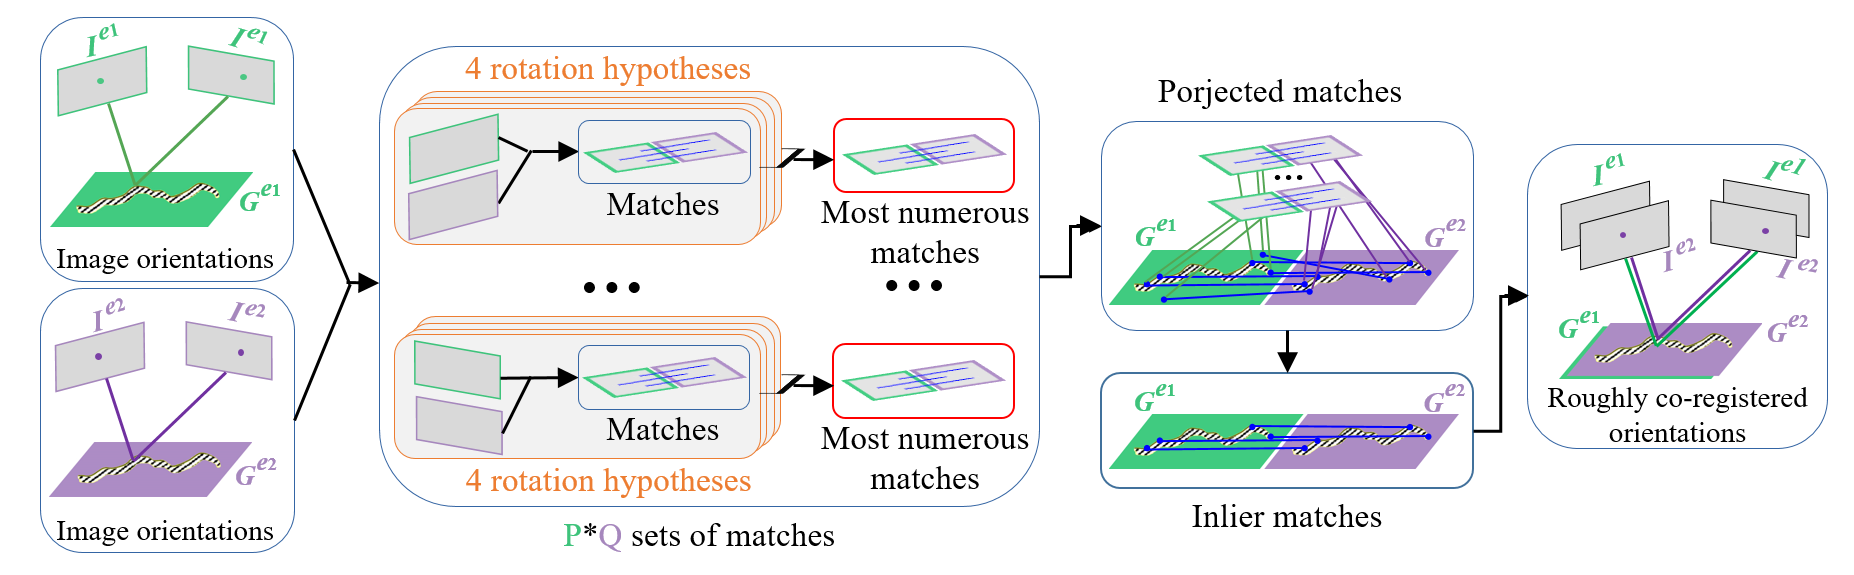
\includegraphics[width=1\columnwidth]{images/Chapitre3/R3D.png}
		\caption{Rough co-registration by matching image pairs.}
		\label{Flow-process diagram}
	\end{center}
\end{figure*}

\subsubsection{SIFT}
\subsubsection{SuperGlue}
\subsection{Strategy 2: Matching DSMs/Orthophotos}
%\subsection{trategy 2: global matching}
\begin{figure*}[htbp]
	\begin{center}
		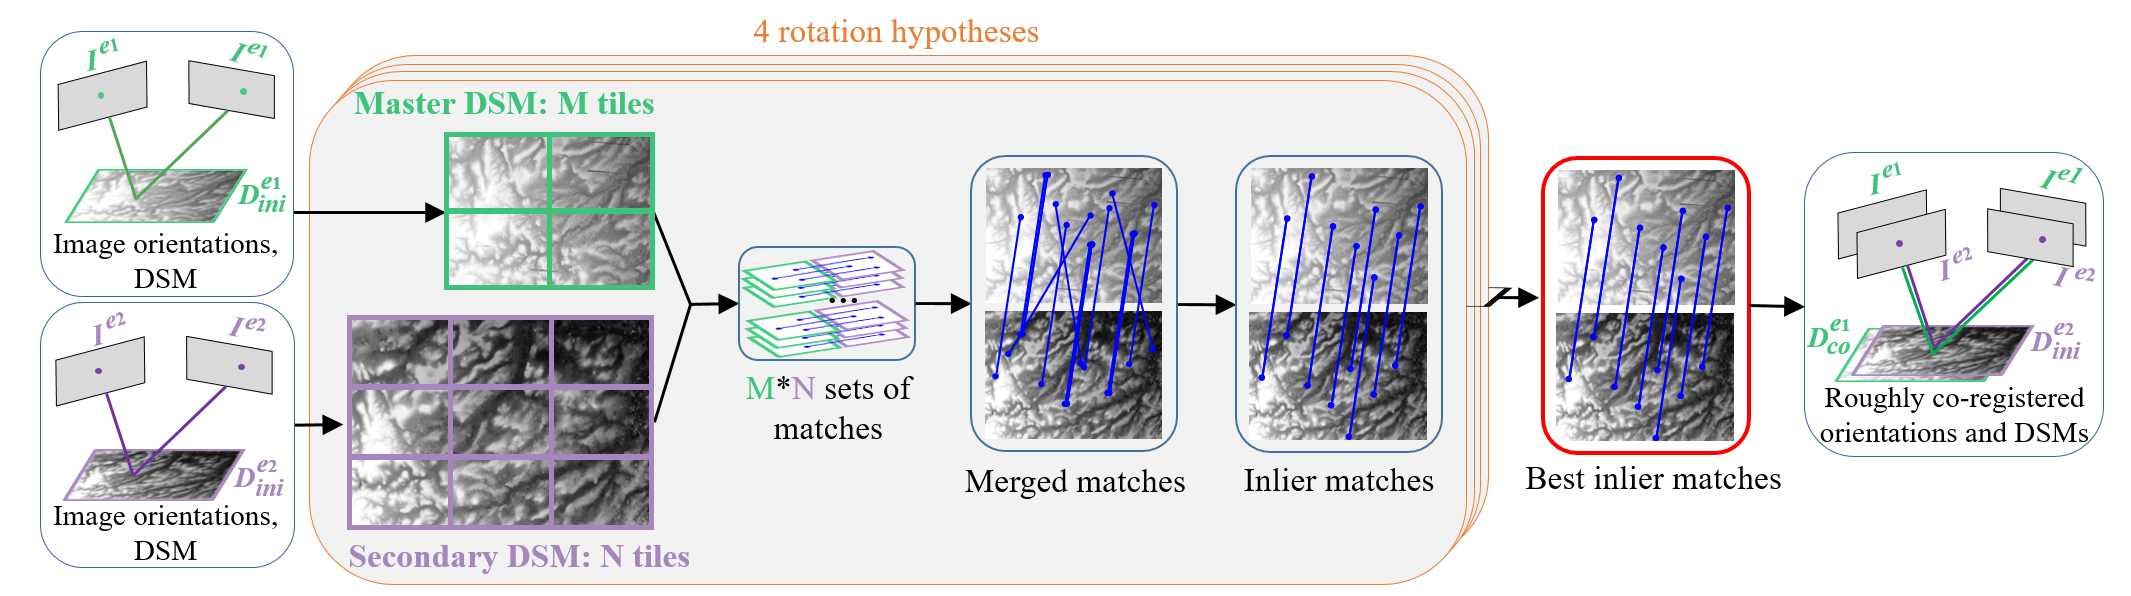
\includegraphics[width=1\columnwidth]{images/Chapitre3/dsm.png}
		\caption{Rough co-registration by matching DSMs.}
		\label{Flow-process diagram}
	\end{center}
\end{figure*}

\begin{figure*}[htbp]
	\begin{center}
		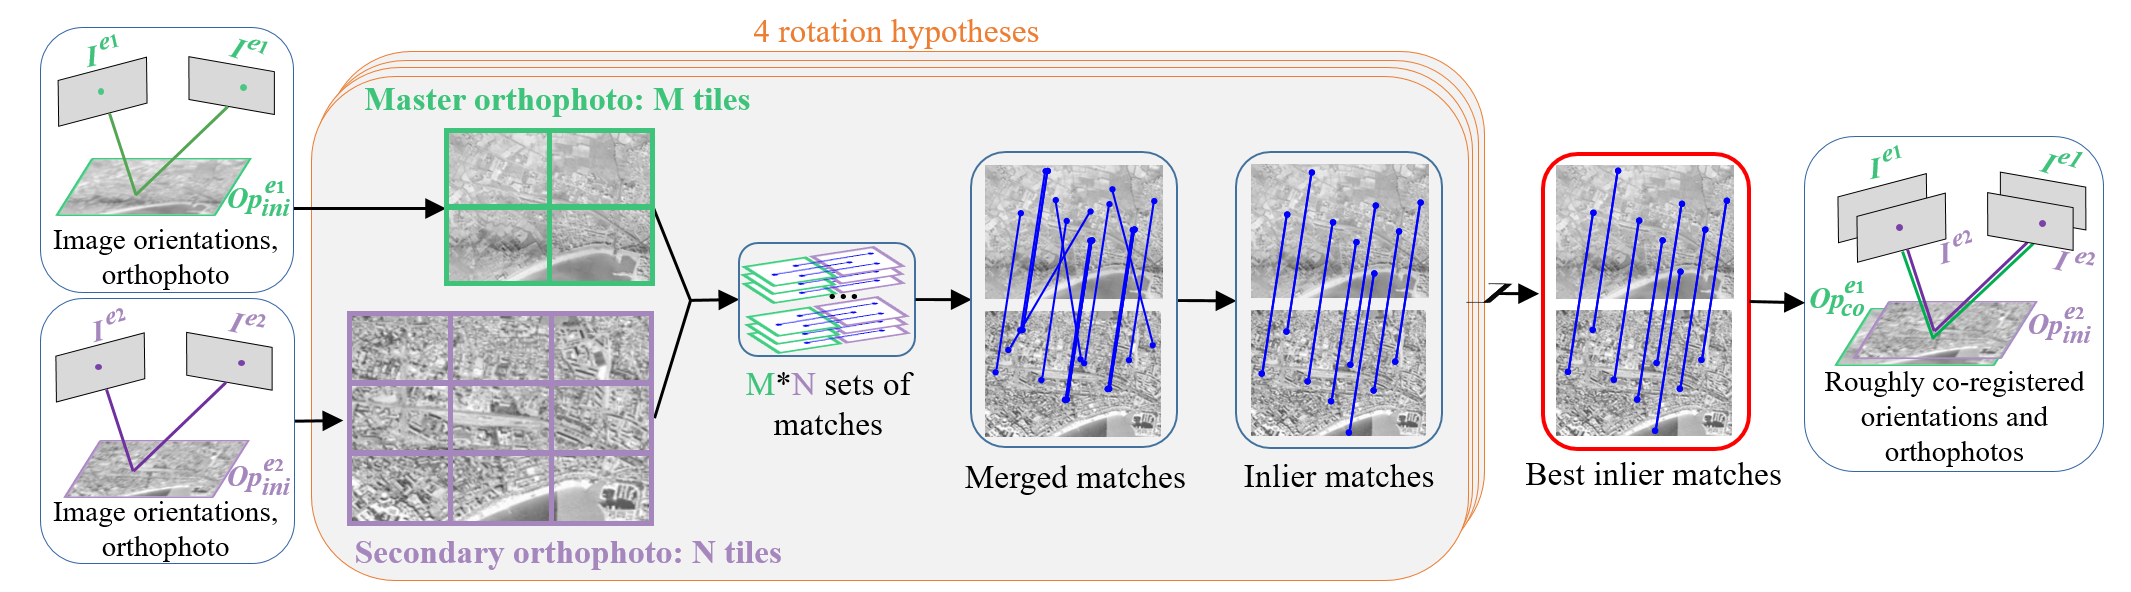
\includegraphics[width=1\columnwidth]{images/Chapitre3/ortho.png}
		\caption{Rough co-registration by matching orthophotos.}
		\label{Flow-process diagram}
	\end{center}
\end{figure*}

\subsubsection{SIFT}
\subsubsection{SuperGlue}

\section{Experiments}
\subsection{Datasets}
Frejus, Pezenas, Kobe\\
%Show piled image of each epoch?
\subsection{Evaluation}

%\subsubsection{Qualitative evaluation}
%\subsubsection{Quantitative evaluation}
(1)Matches visualization\\
%inlier ratio (RANSAC and GT)\\
(2)Ground check points\\
(3)DoD\\

\subsection{Comparison}
%分三部分分别展示3组数据的结果
%3*2 methods:
%1张表表示6种方法的(1)和(2),1张大图放6种方法的DoD, inlier tie pt图(R3D, DSM, ortho各3张(无点图,SIFT点图,SpG点图))

\subsubsection{Matches visualization}

\begin{figure*}[htbp]
	\begin{center}
		\subfigure[Image pairs]{
			\begin{minipage}[t]{0.65\linewidth}
				\centering
				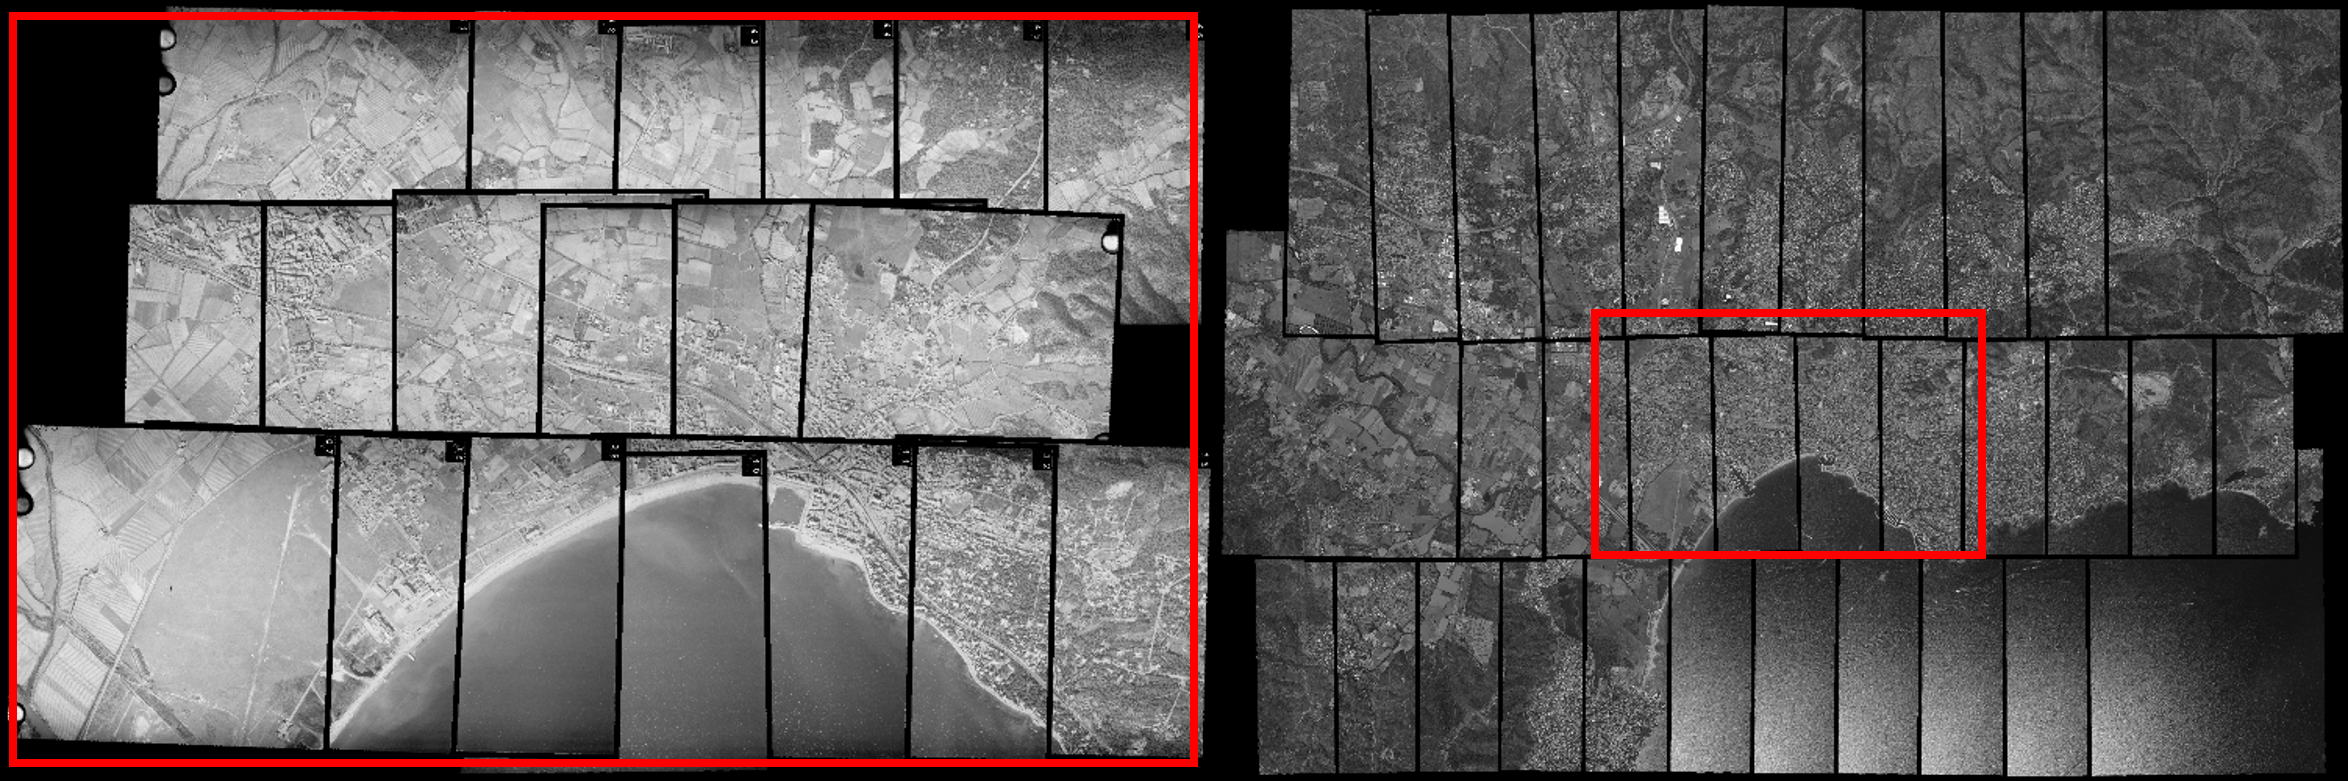
\includegraphics[width=8.8cm]{images/Chapitre3/Pseudo-Ortho-MEC-Malt_Tapas_1954_Ortho-MEC-Malt_2014.png}
			\end{minipage}%
		}
		\subfigure[Match number (ImgPairs)]{
	\begin{minipage}[t]{0.3\linewidth}
		\centering
		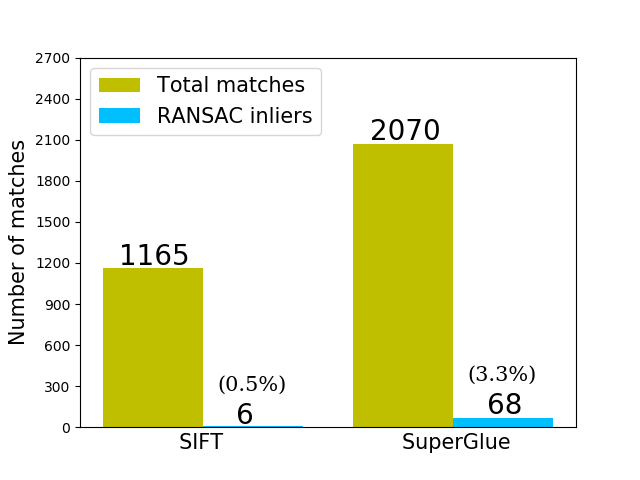
\includegraphics[width=4.8cm]{images/Chapitre3/PlotCurves_Pseudo-Ortho-MEC-Malt_Tapas_1954_Ortho-MEC-Malt_2014.png}
	\end{minipage}%
}
		\subfigure[$SIFT_{ImgPairs}$]{
			\begin{minipage}[t]{0.48\linewidth}
				\centering
				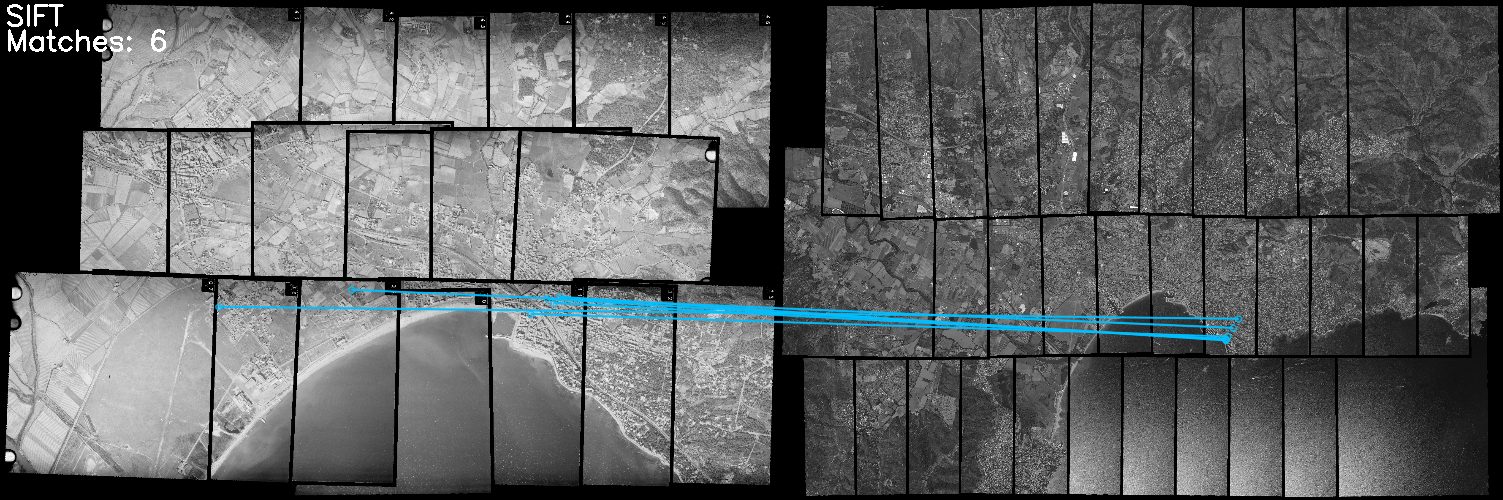
\includegraphics[width=6.8cm]{images/Chapitre3/Pseudo-Homol-SIFT2Step_1954-2014-Rough-2DRANSAC-GlobalR3D-PileImg_Ortho-MEC-Malt_Tapas_1954_Ortho-MEC-Malt_2014.png}
			\end{minipage}%
		}
		\subfigure[$SuperGlue_{ImgPairs}$]{
			\begin{minipage}[t]{0.48\linewidth}
				\centering
				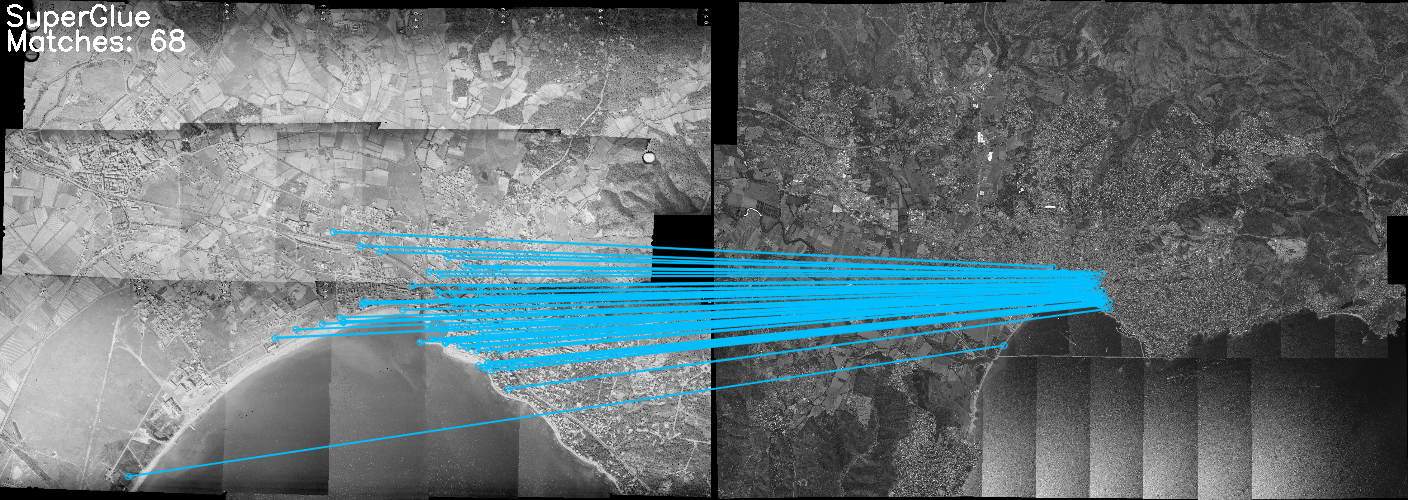
\includegraphics[width=6.8cm]{images/Chapitre3/Pseudo-Homol-SuperGlue_1954-2014-GlobalR3D-PileImg_Ortho-MEC-Malt_Tapas_1954_Ortho-MEC-Malt_2014.png}
			\end{minipage}%
		}
		\caption{Result of matching image pairs of Fr{\'e}jus 1954 and 2014}
		\label{Match result}
	\end{center}
\end{figure*} 



\begin{figure*}[htbp]
	\begin{center}
		\subfigure[Orthophotos]{
	\begin{minipage}[t]{0.65\linewidth}
		\centering
		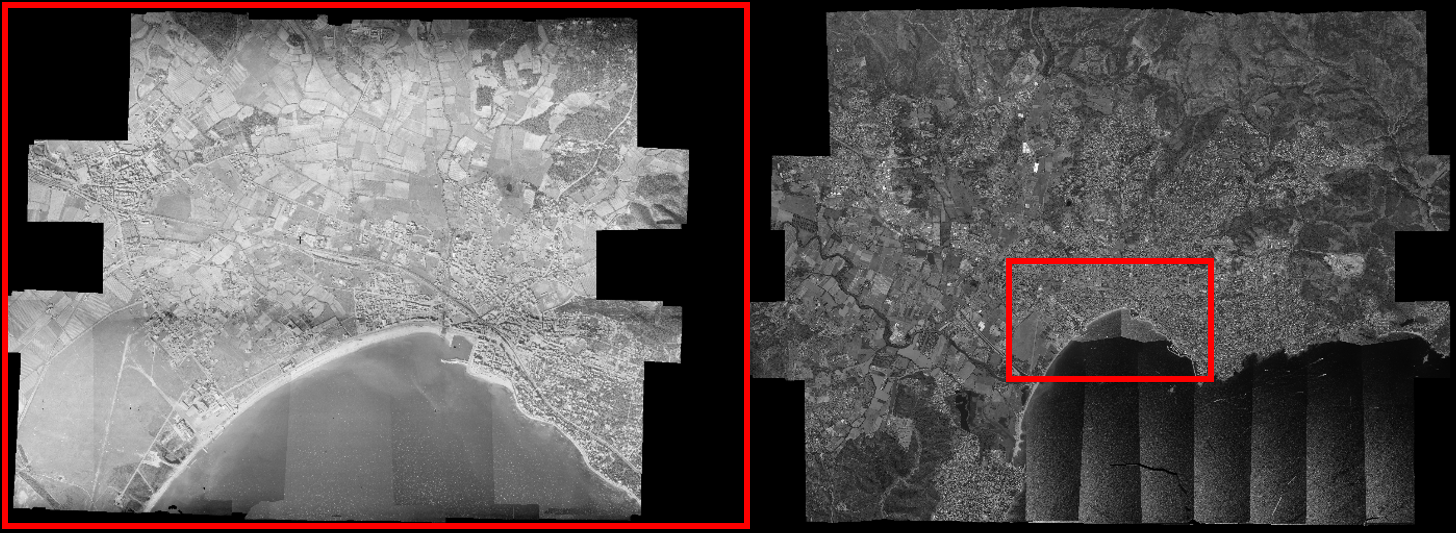
\includegraphics[width=8.8cm]{images/Chapitre3/Ortho-MEC-Malt_Tapas_1954_Ortho-MEC-Malt_2014.png}
	\end{minipage}%
}
\subfigure[Match number (ortho)]{
	\begin{minipage}[t]{0.3\linewidth}
		\centering
		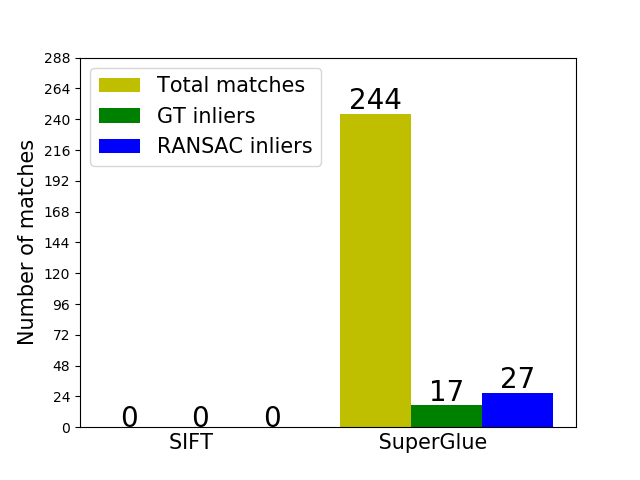
\includegraphics[width=4.8cm]{images/Chapitre3/PlotCurves_Ortho-MEC-Malt_Tapas_1954_Ortho-MEC-Malt_2014.png}
	\end{minipage}%
}
		\subfigure[$SIFT_{ortho}$]{
			\begin{minipage}[t]{0.48\linewidth}
				\centering
				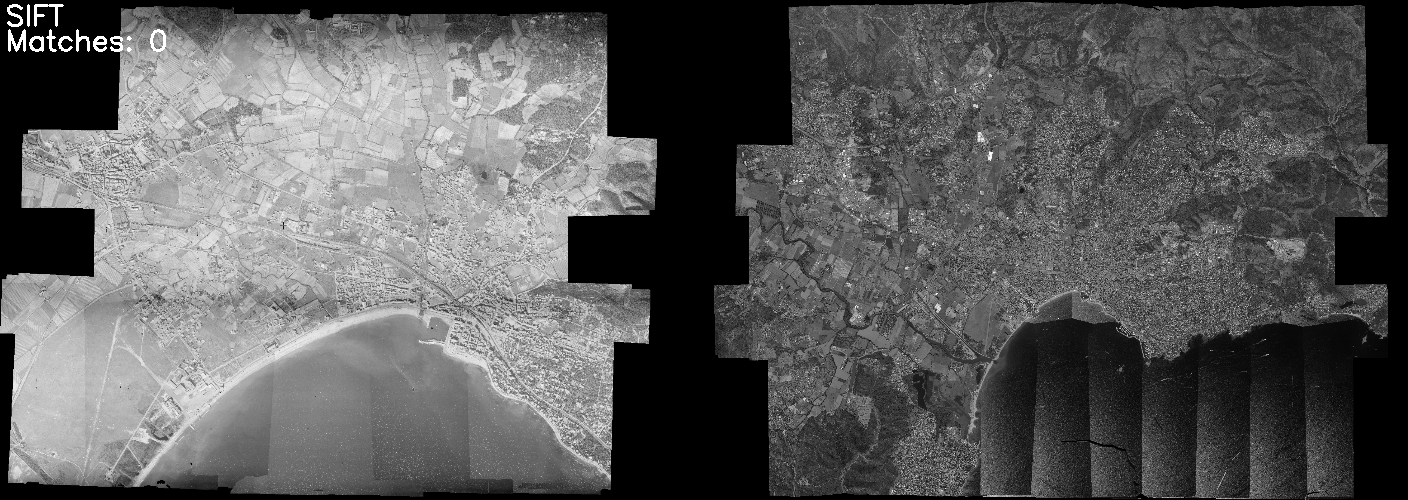
\includegraphics[width=6.8cm]{images/Chapitre3/Homol-SIFT-2DRANSAC_Ortho-MEC-Malt_Tapas_1954_Ortho-MEC-Malt_2014.png}
			\end{minipage}%
		}
		\subfigure[$SuperGlue_{ortho}$]{
			\begin{minipage}[t]{0.48\linewidth}
				\centering
				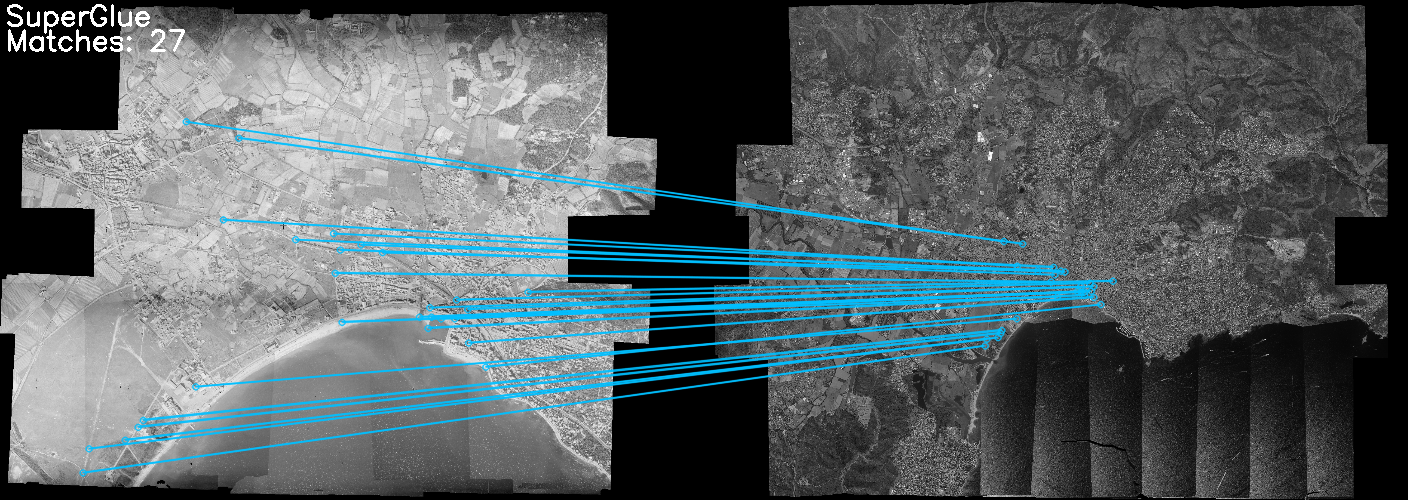
\includegraphics[width=6.8cm]{images/Chapitre3/Homol-SubPatch_R270-2DRANSAC_Ortho-MEC-Malt_Tapas_1954_Ortho-MEC-Malt_2014.png}
			\end{minipage}%
		}
		\caption{Result of matching orthophotos of Fr{\'e}jus 1954 and 2014}
		\label{Match result}
	\end{center}
\end{figure*} 

\begin{figure*}[htbp]
	\begin{center}
		\subfigure[DSMs]{
	\begin{minipage}[t]{0.65\linewidth}
		\centering
		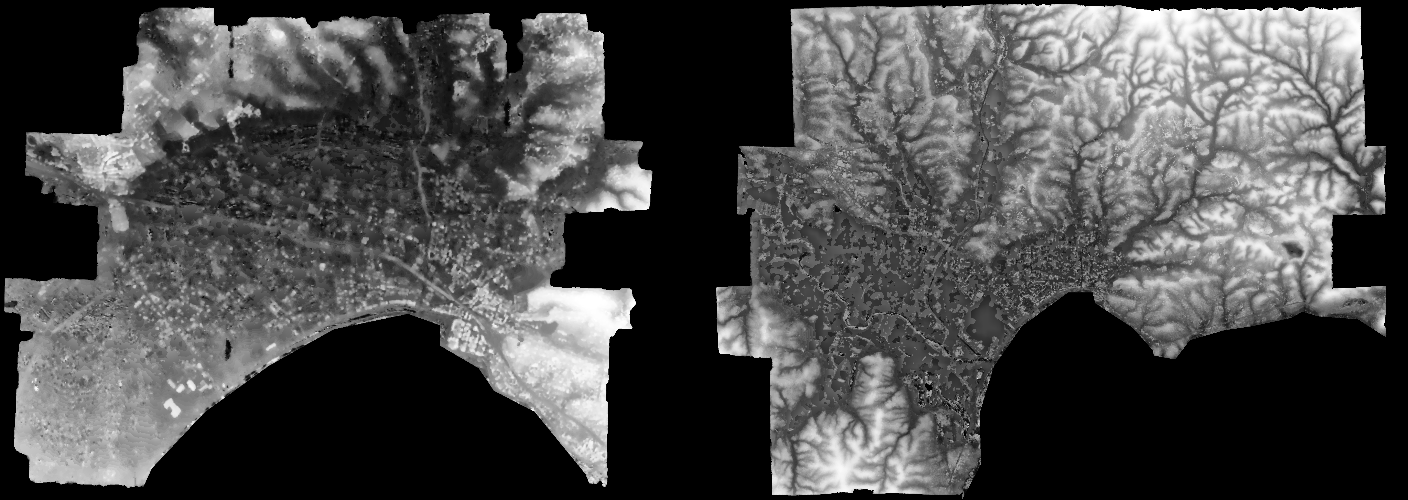
\includegraphics[width=8.8cm]{images/Chapitre3/MEC-Malt_Tapas_1954_MEC-Malt_2014.png}
	\end{minipage}%
}
\subfigure[Match number (DSM)]{
	\begin{minipage}[t]{0.3\linewidth}
		\centering
		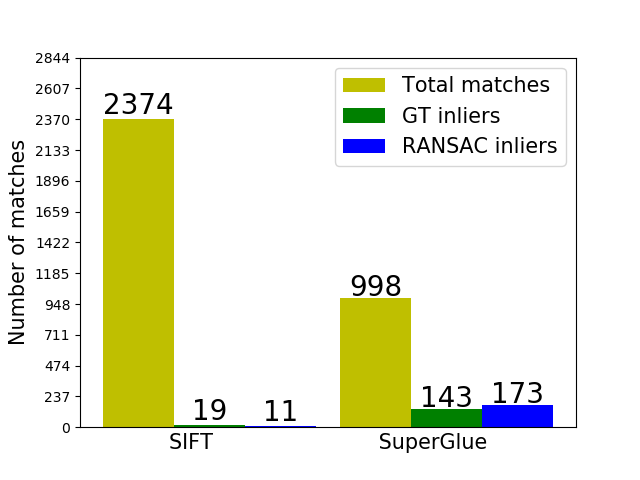
\includegraphics[width=4.8cm]{images/Chapitre3/PlotCurves_MEC-Malt_Tapas_1954_MEC-Malt_2014.png}
	\end{minipage}%
}
		\subfigure[$SIFT_{DSM}$]{
			\begin{minipage}[t]{0.48\linewidth}
				\centering
				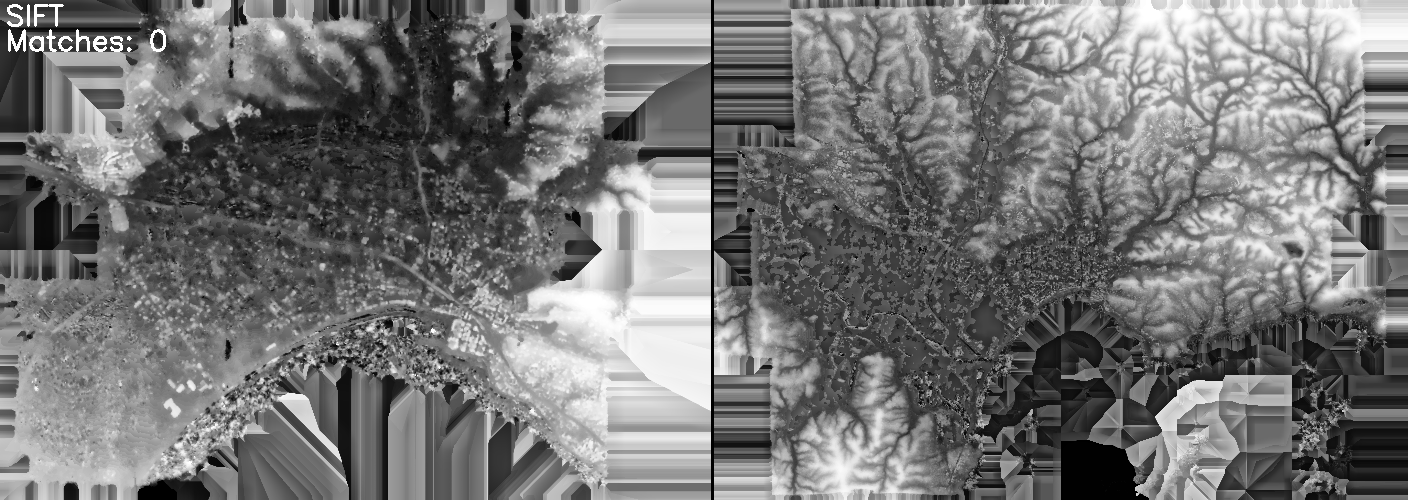
\includegraphics[width=6.8cm]{images/Chapitre3/Homol-SIFT-2DRANSAC_MEC-Malt_Tapas_1954_MEC-Malt_2014.png}
			\end{minipage}%
		}
		\subfigure[$SuperGlue_{DSM}$]{
			\begin{minipage}[t]{0.48\linewidth}
				\centering
				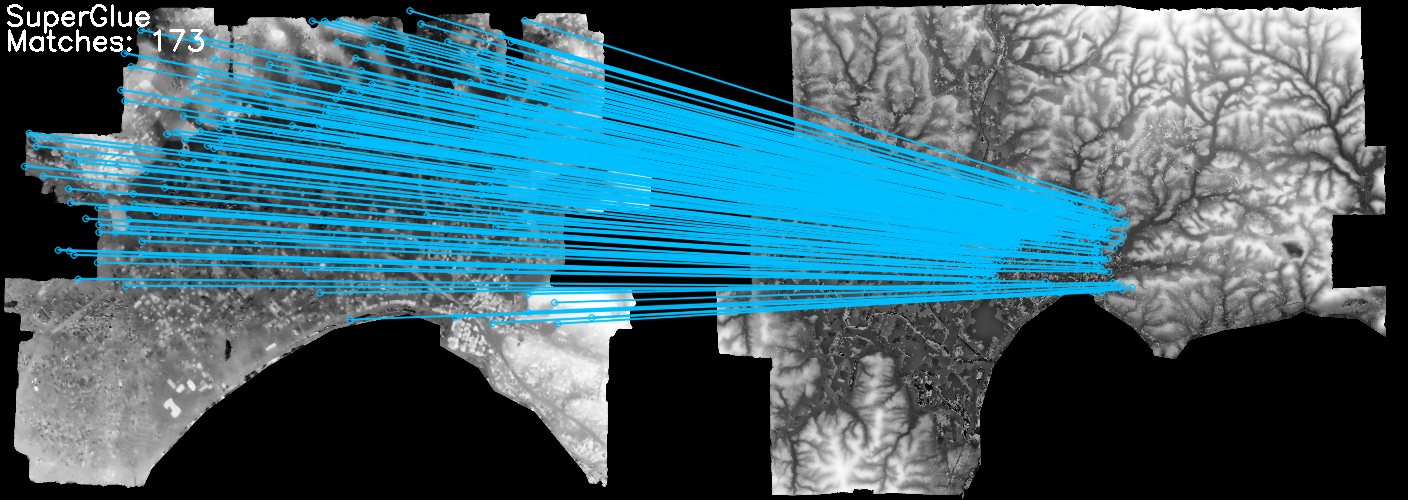
\includegraphics[width=6.8cm]{images/Chapitre3/Homol-SubPatch_R270-2DRANSAC_MEC-Malt_Tapas_1954_MEC-Malt_2014.png}
			\end{minipage}%
		}
		\caption{Result of matching DSMs of Fr{\'e}jus 1954 and 2014}
		\label{Match result}
	\end{center}
\end{figure*} 



\begin{figure*}[htbp]
	\begin{center}
		\subfigure[Image pairs]{
			\begin{minipage}[t]{0.65\linewidth}
				\centering
				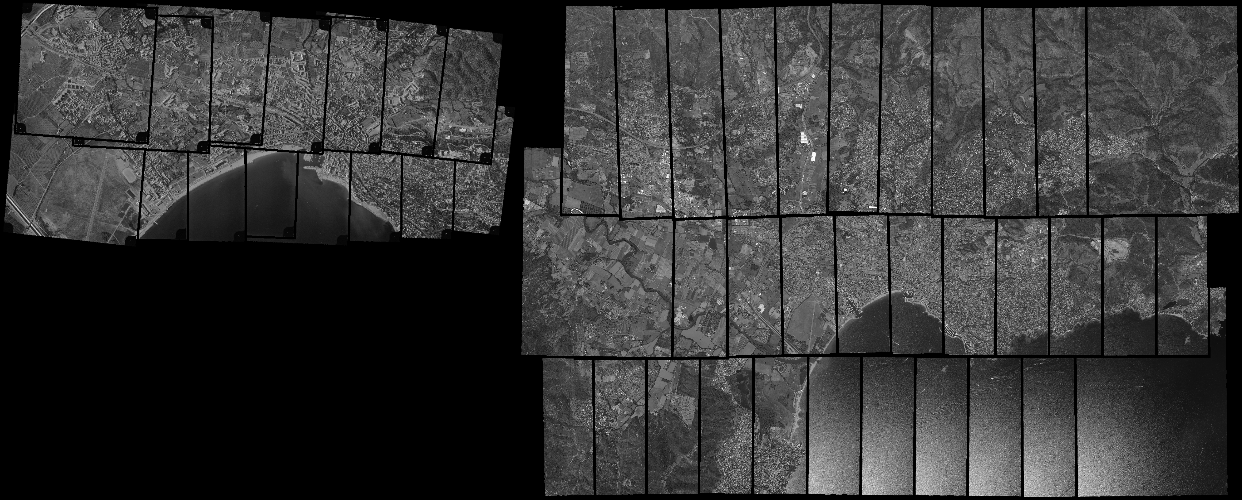
\includegraphics[width=8.1cm]{images/Chapitre3/Pseudo-Ortho-MEC-Malt_Tapas_1966_Ortho-MEC-Malt_2014.png}
			\end{minipage}%
		}
		\subfigure[Match number (ImgPairs)]{
			\begin{minipage}[t]{0.3\linewidth}
				\centering
				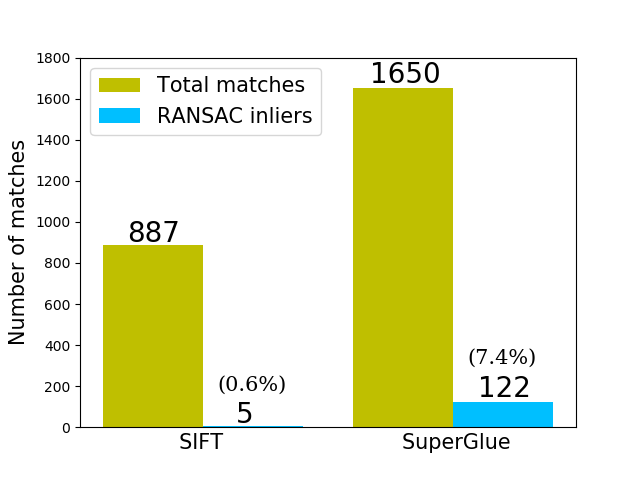
\includegraphics[width=4.8cm]{images/Chapitre3/PlotCurves_Pseudo-Ortho-MEC-Malt_Tapas_1966_Ortho-MEC-Malt_2014.png}
			\end{minipage}%
		}
		\subfigure[$SIFT_{ImgPairs}$]{
			\begin{minipage}[t]{0.48\linewidth}
				\centering
				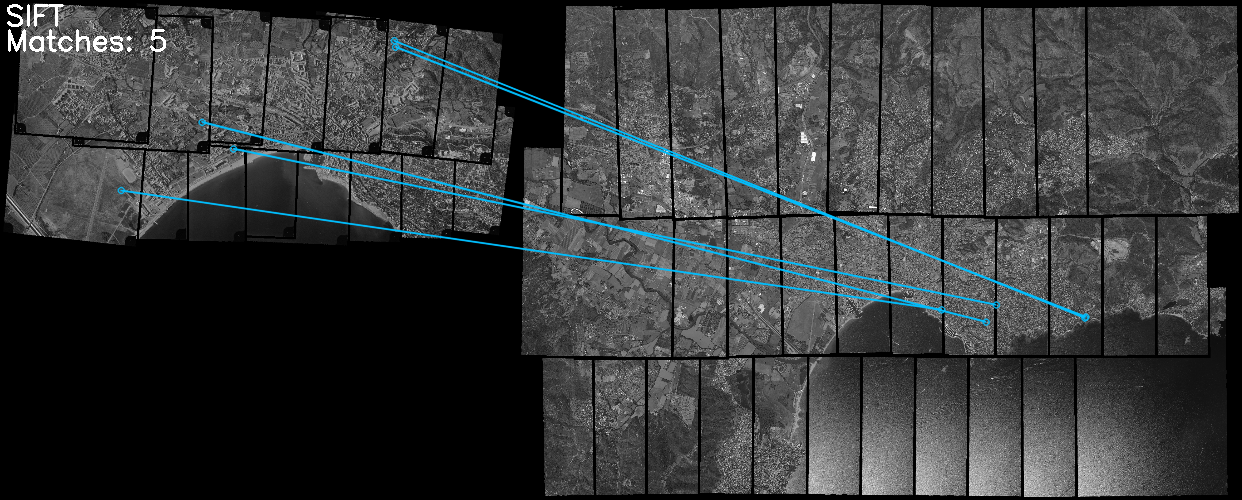
\includegraphics[width=6cm]{images/Chapitre3/Pseudo-Homol-SIFT2Step_1966-2014-Rough-2DRANSAC-GlobalR3D-PileImg_Ortho-MEC-Malt_Tapas_1966_Ortho-MEC-Malt_2014.png}
			\end{minipage}%
		}
		\subfigure[$SuperGlue_{ImgPairs}$]{
			\begin{minipage}[t]{0.48\linewidth}
				\centering
				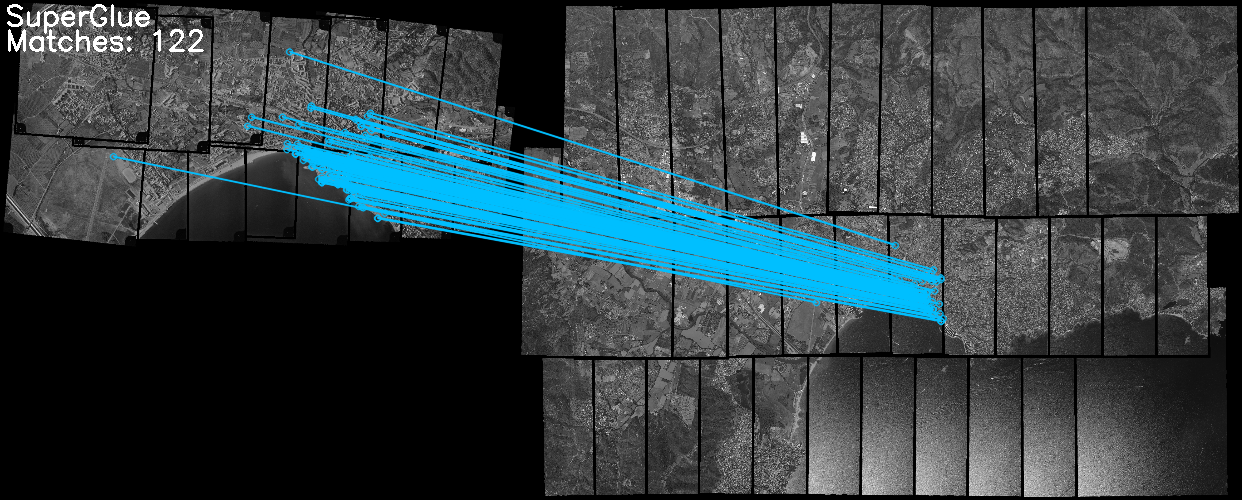
\includegraphics[width=6cm]{images/Chapitre3/Pseudo-Homol-SuperGlue_1966-2014-GlobalR3D-PileImg_Ortho-MEC-Malt_Tapas_1966_Ortho-MEC-Malt_2014.png}
			\end{minipage}%
		}
		\caption{Result of matching image pairs of Fr{\'e}jus 1966 and 2014}
		\label{Match result}
	\end{center}
\end{figure*} 


\begin{figure*}[htbp]
	\begin{center}
		\subfigure[Orthophotos]{
			\begin{minipage}[t]{0.65\linewidth}
				\centering
				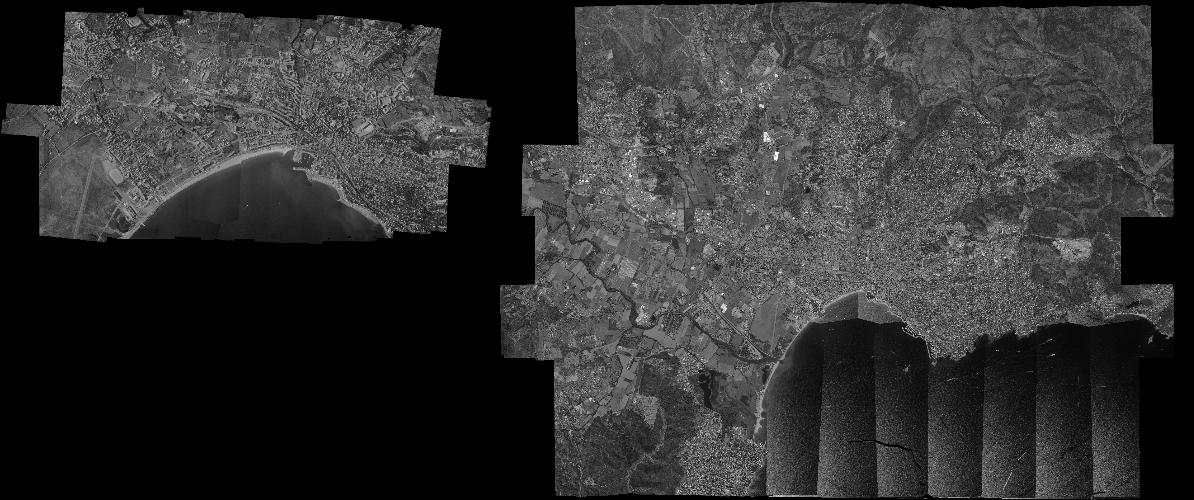
\includegraphics[width=8.1cm]{images/Chapitre3/Ortho-MEC-Malt_Tapas_1966_Ortho-MEC-Malt_2014.png}
			\end{minipage}%
		}
		\subfigure[Match number (ortho)]{
			\begin{minipage}[t]{0.3\linewidth}
				\centering
				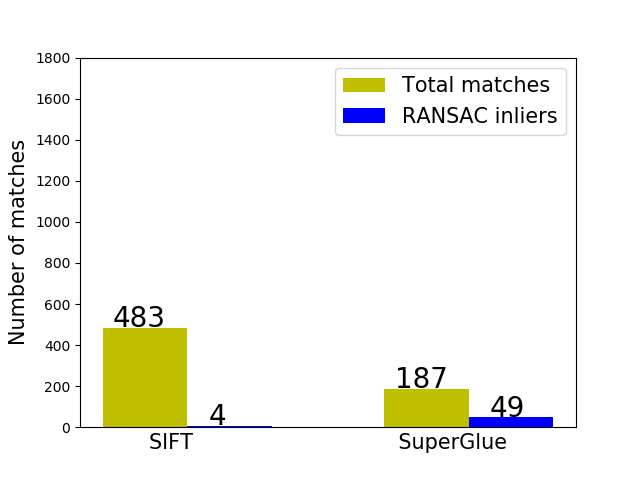
\includegraphics[width=4.8cm]{images/Chapitre3/PlotCurves_Ortho-MEC-Malt_Tapas_1966_Ortho-MEC-Malt_2014.png}
			\end{minipage}%
		}
		\subfigure[$SIFT_{ortho}$]{
			\begin{minipage}[t]{0.48\linewidth}
				\centering
				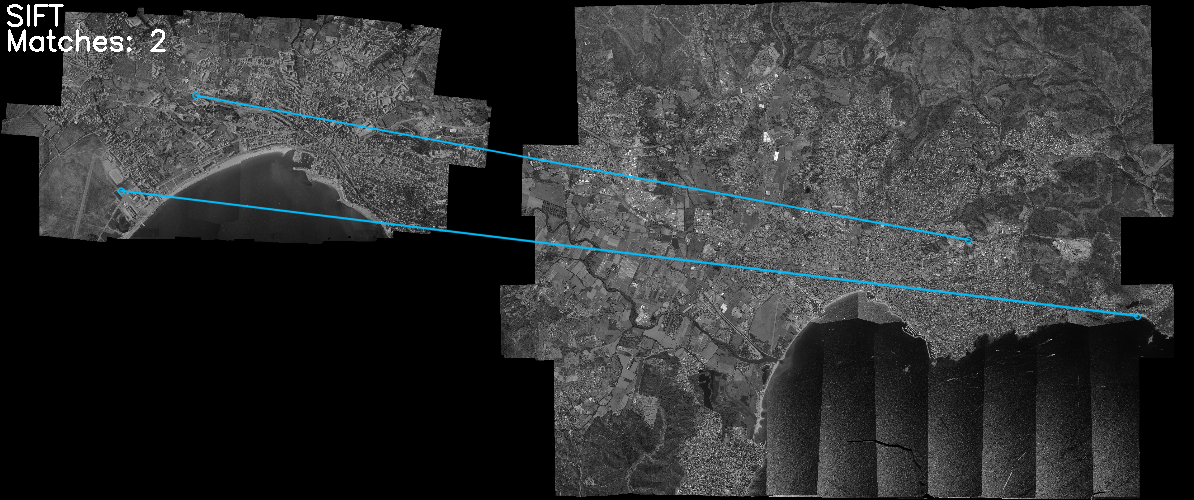
\includegraphics[width=6cm]{images/Chapitre3/Homol-SIFT-2DRANSAC_Ortho-MEC-Malt_Tapas_1966_Ortho-MEC-Malt_2014.png}
			\end{minipage}%
		}
		\subfigure[$SuperGlue_{ortho}$]{
			\begin{minipage}[t]{0.48\linewidth}
				\centering
				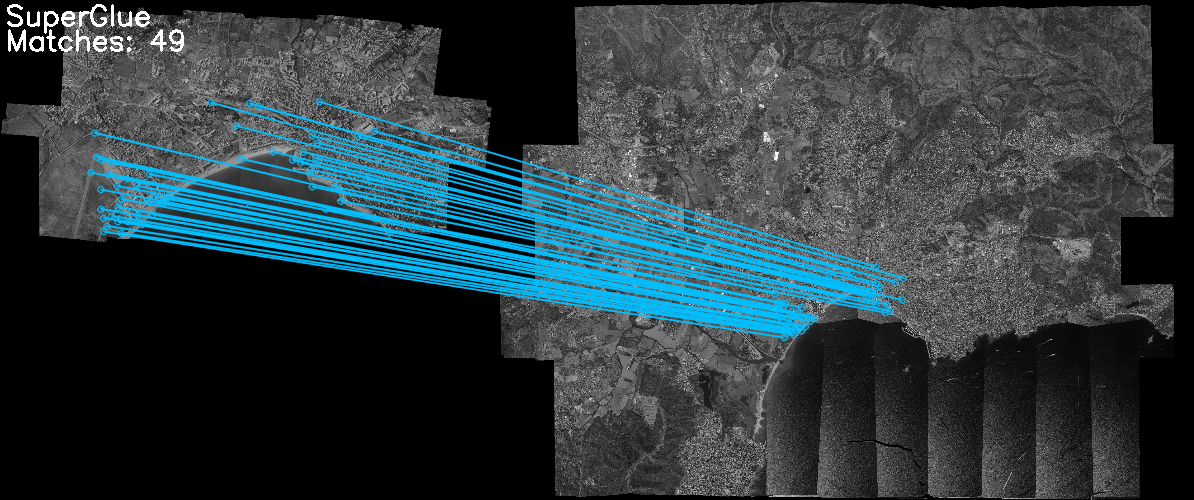
\includegraphics[width=6cm]{images/Chapitre3/Homol-SubPatch_R270-2DRANSAC_Ortho-MEC-Malt_Tapas_1966_Ortho-MEC-Malt_2014.png}
			\end{minipage}%
		}
		\caption{Result of matching orthophotos of Fr{\'e}jus 1966 and 2014}
		\label{Match result}
	\end{center}
\end{figure*} 

\begin{figure*}[htbp]
	\begin{center}
		\subfigure[DSMs]{
			\begin{minipage}[t]{0.65\linewidth}
				\centering
				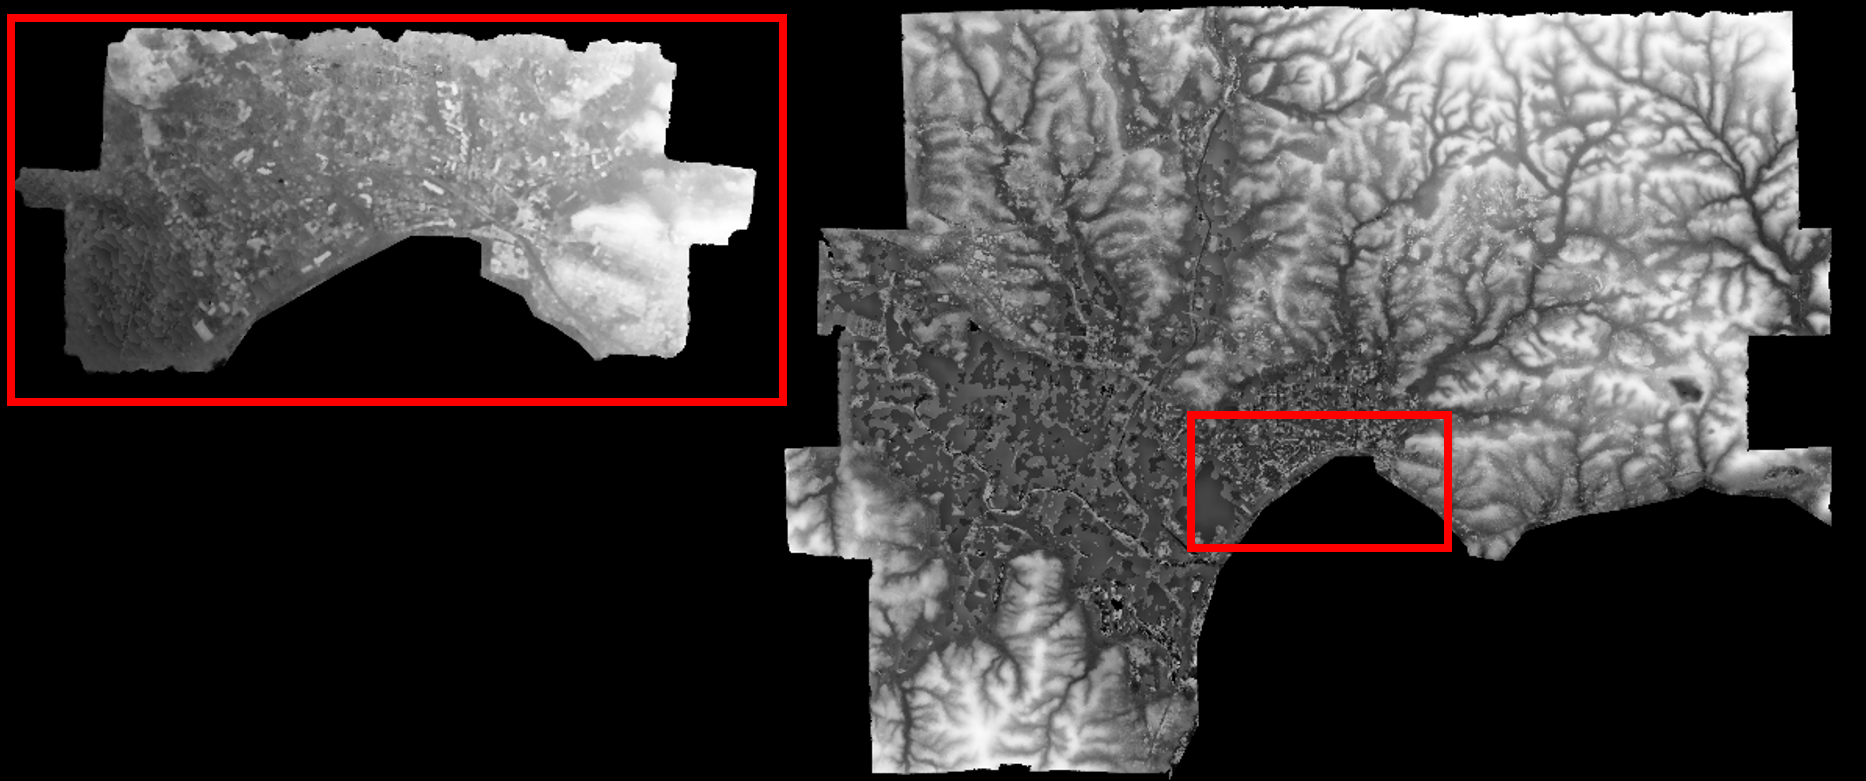
\includegraphics[width=8.1cm]{images/Chapitre3/MEC-Malt_Tapas_1966_MEC-Malt_2014.png}
			\end{minipage}%
		}
		\subfigure[Match number (DSM)]{
			\begin{minipage}[t]{0.3\linewidth}
				\centering
				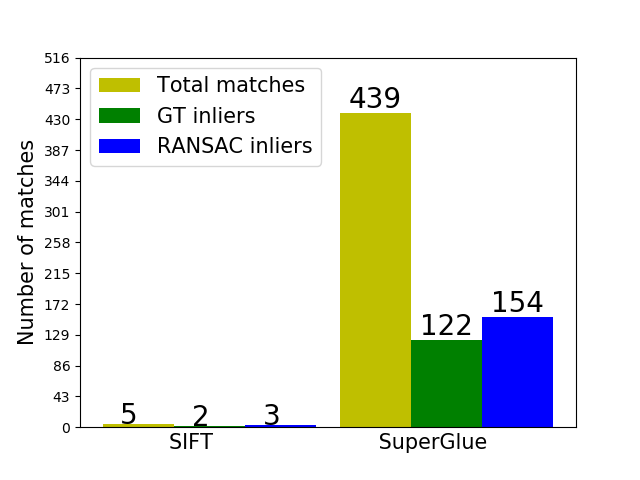
\includegraphics[width=4.8cm]{images/Chapitre3/PlotCurves_MEC-Malt_Tapas_1966_MEC-Malt_2014.png}
			\end{minipage}%
		}
		\subfigure[$SIFT_{DSM}$]{
			\begin{minipage}[t]{0.48\linewidth}
				\centering
				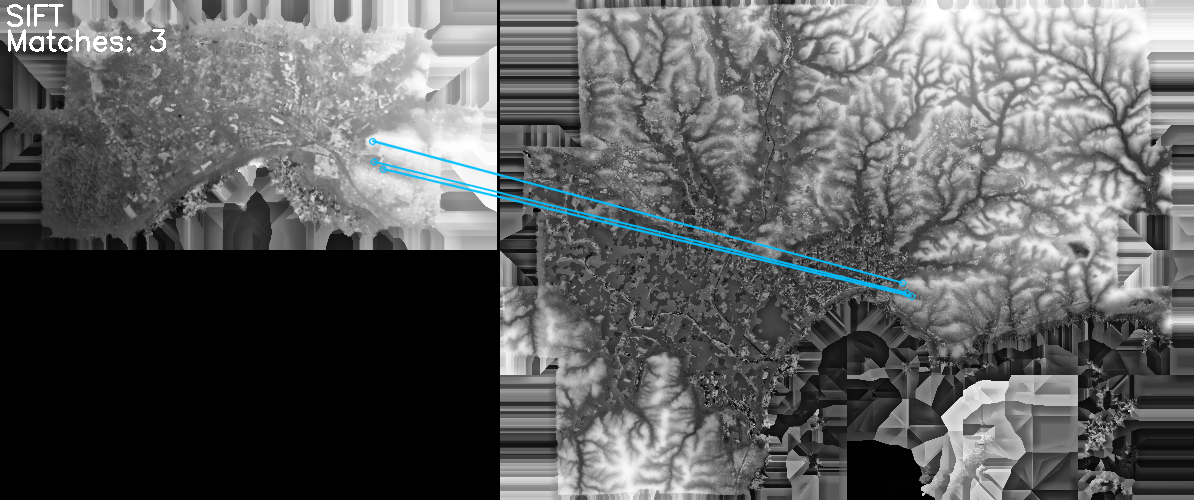
\includegraphics[width=6cm]{images/Chapitre3/Homol-SIFT-2DRANSAC_MEC-Malt_Tapas_1966_MEC-Malt_2014.png}
			\end{minipage}%
		}
		\subfigure[$SuperGlue_{DSM}$]{
			\begin{minipage}[t]{0.48\linewidth}
				\centering
				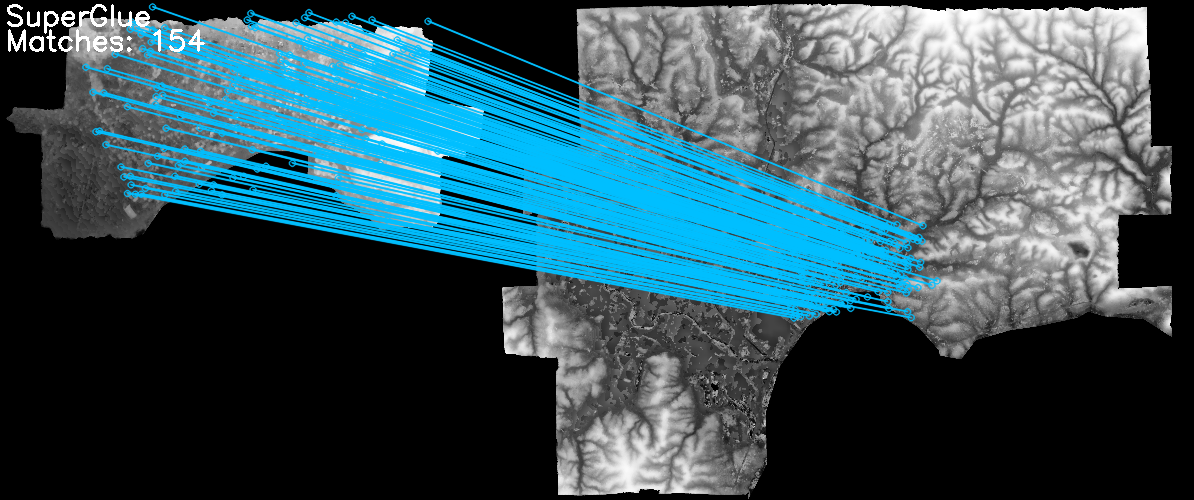
\includegraphics[width=6cm]{images/Chapitre3/Homol-SubPatch_R270-2DRANSAC_MEC-Malt_Tapas_1966_MEC-Malt_2014.png}
			\end{minipage}%
		}
		\caption{Result of matching DSMs of Fr{\'e}jus 1966 and 2014}
		\label{Match result}
	\end{center}
\end{figure*} 






\begin{figure*}[htbp]
	\begin{center}
		\subfigure[Image pairs]{
			\begin{minipage}[t]{0.6\linewidth}
				\centering
				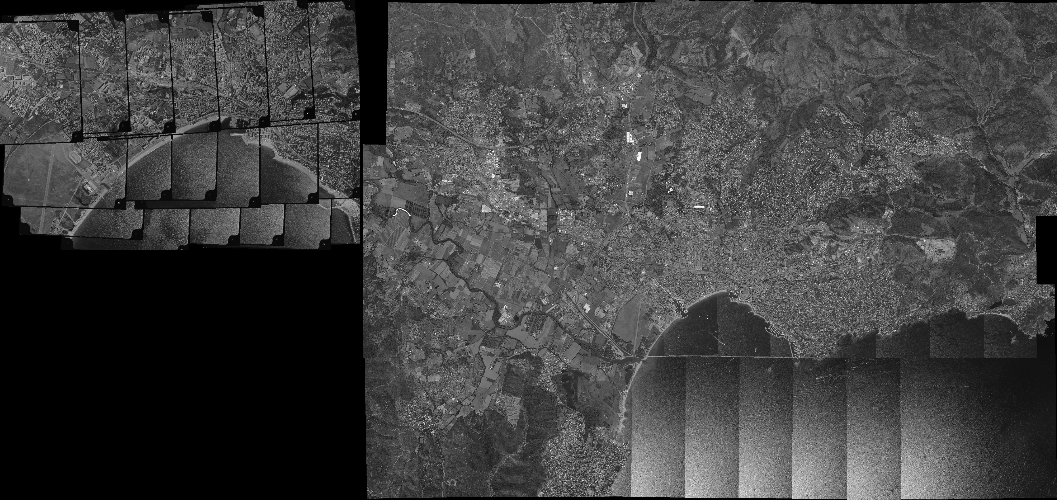
\includegraphics[width=7.8cm]{images/Chapitre3/Pseudo-Ortho-MEC-Malt_Tapas_1970_Ortho-MEC-Malt_2014.png}
			\end{minipage}%
		}
		\subfigure[Match number (ImgPairs)]{
			\begin{minipage}[t]{0.35\linewidth}
				\centering
				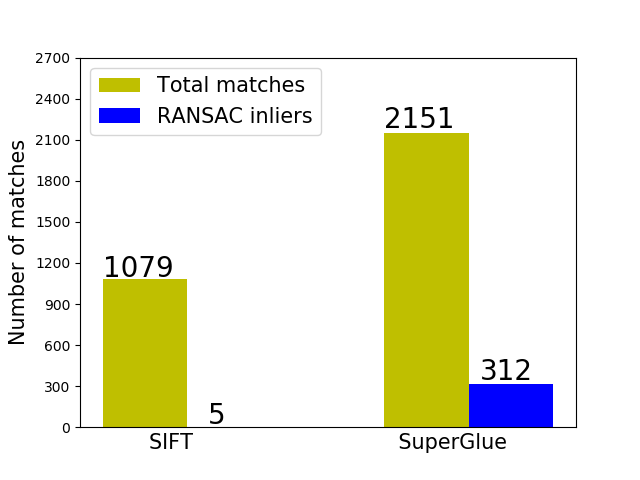
\includegraphics[width=4.8cm]{images/Chapitre3/PlotCurves_Pseudo-Ortho-MEC-Malt_Tapas_1970_Ortho-MEC-Malt_2014.png}
			\end{minipage}%
		}
		\subfigure[$SIFT_{ImgPairs}$]{
			\begin{minipage}[t]{0.48\linewidth}
				\centering
				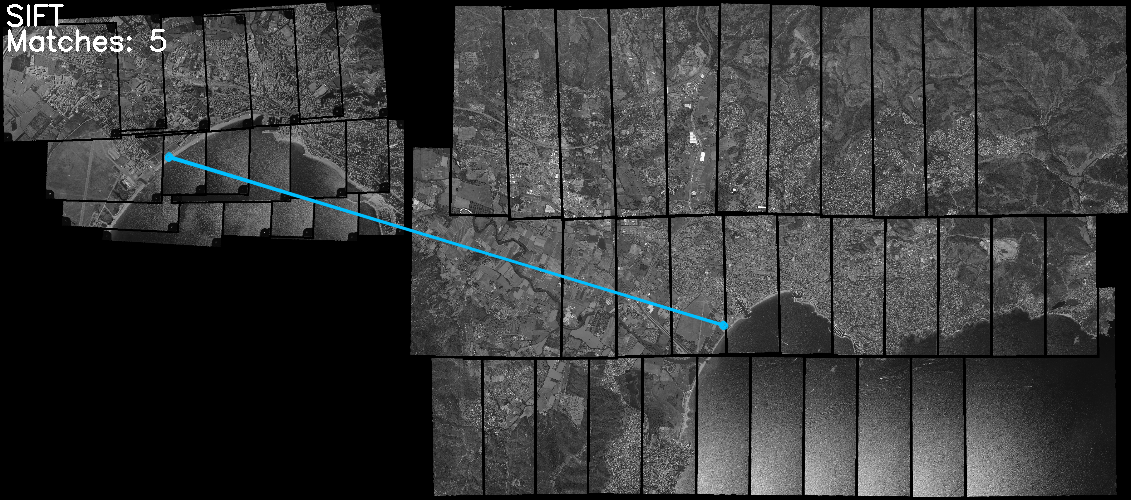
\includegraphics[width=6cm]{images/Chapitre3/Pseudo-Homol-SIFT2Step_1970-2014-Rough-2DRANSAC-GlobalR3D-PileImg_Ortho-MEC-Malt_Tapas_1970_Ortho-MEC-Malt_2014.png}
			\end{minipage}%
		}
		\subfigure[$SuperGlue_{ImgPairs}$]{
			\begin{minipage}[t]{0.48\linewidth}
				\centering
				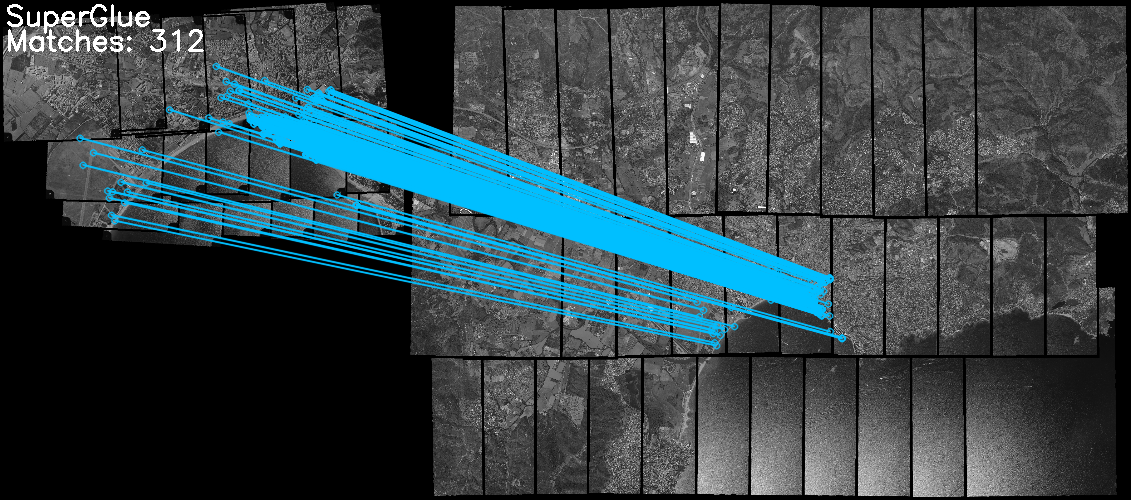
\includegraphics[width=6cm]{images/Chapitre3/Pseudo-Homol-SuperGlue_1970-2014-GlobalR3D-PileImg_Ortho-MEC-Malt_Tapas_1970_Ortho-MEC-Malt_2014.png}
			\end{minipage}%
		}
		\caption{Result of matching image pairs of Fr{\'e}jus 1970 and 2014}
		\label{Match result}
	\end{center}
\end{figure*} 

\begin{figure*}[htbp]
	\begin{center}
		\subfigure[Orthophotos]{
			\begin{minipage}[t]{0.6\linewidth}
				\centering
				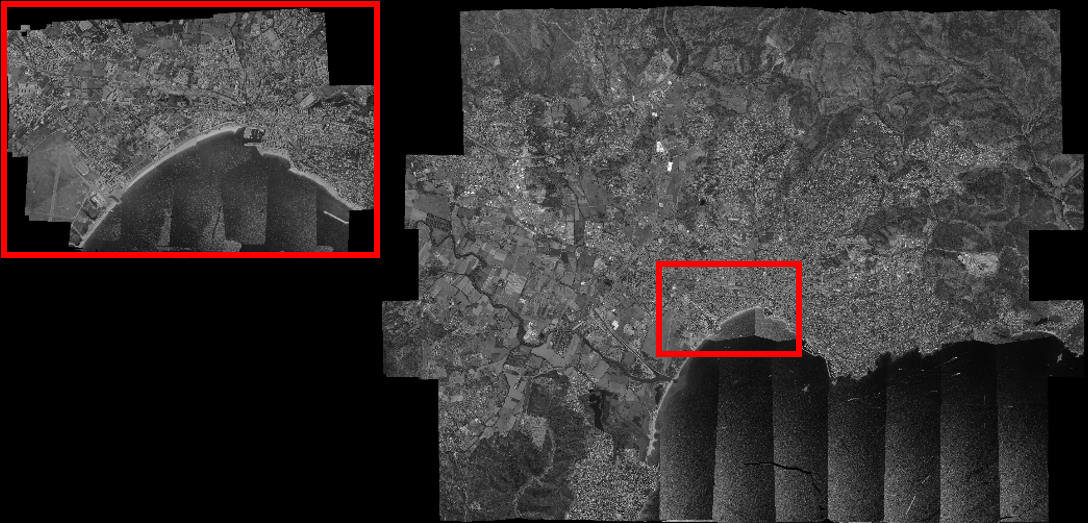
\includegraphics[width=7.8cm]{images/Chapitre3/Ortho-MEC-Malt_Tapas_1970_Ortho-MEC-Malt_2014.png}
			\end{minipage}%
		}
		\subfigure[Match number (ortho)]{
			\begin{minipage}[t]{0.35\linewidth}
				\centering
				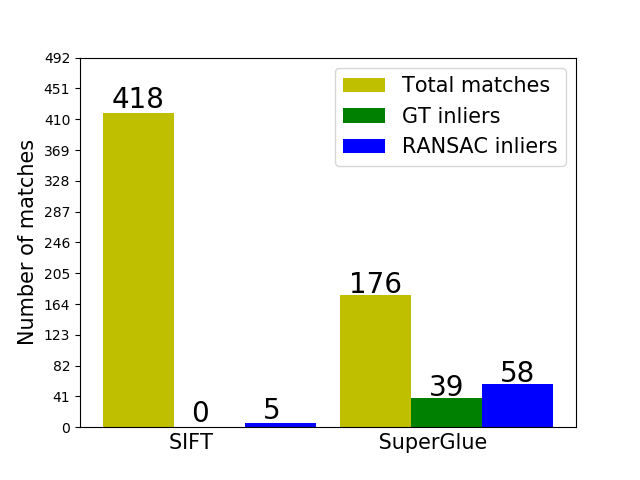
\includegraphics[width=4.8cm]{images/Chapitre3/PlotCurves_Ortho-MEC-Malt_Tapas_1970_Ortho-MEC-Malt_2014.png}
			\end{minipage}%
		}
		\subfigure[$SIFT_{ortho}$]{
			\begin{minipage}[t]{0.48\linewidth}
				\centering
				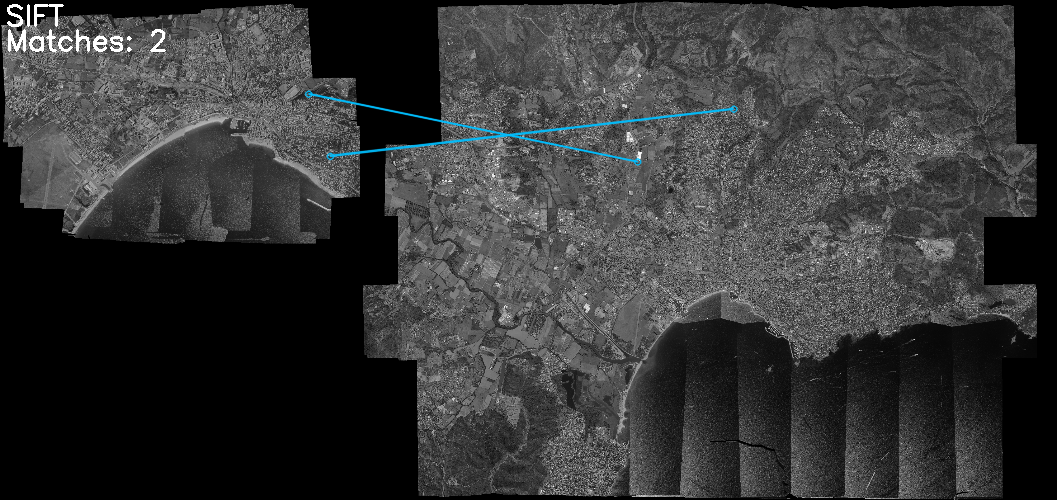
\includegraphics[width=6cm]{images/Chapitre3/Homol-SIFT-2DRANSAC_Ortho-MEC-Malt_Tapas_1970_Ortho-MEC-Malt_2014.png}
			\end{minipage}%
		}
		\subfigure[$SuperGlue_{ortho}$]{
			\begin{minipage}[t]{0.48\linewidth}
				\centering
				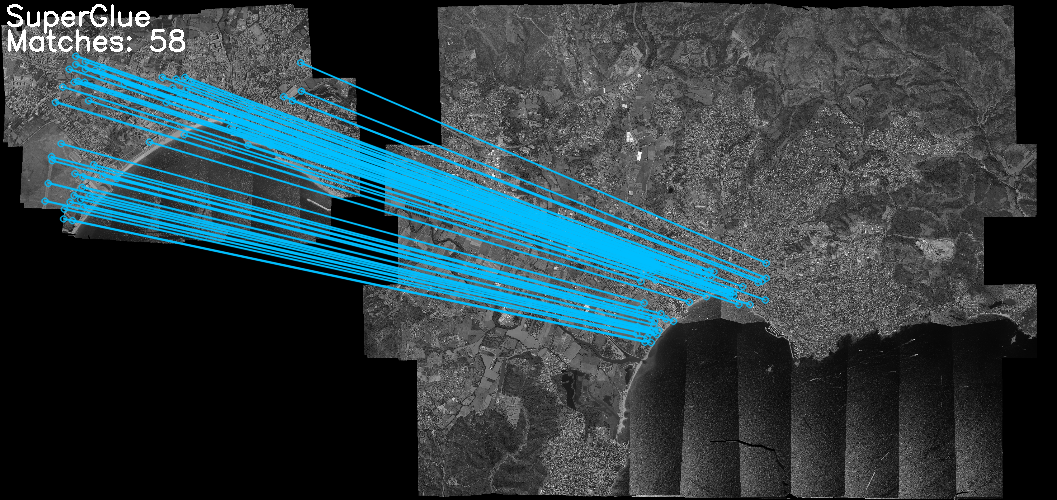
\includegraphics[width=6cm]{images/Chapitre3/Homol-SubPatch_R270-2DRANSAC_Ortho-MEC-Malt_Tapas_1970_Ortho-MEC-Malt_2014.png}
			\end{minipage}%
		}
		\caption{Result of matching orthophotos of Fr{\'e}jus 1970 and 2014}
		\label{Match result}
	\end{center}
\end{figure*} 

\begin{figure*}[htbp]
	\begin{center}
		\subfigure[DSMs]{
			\begin{minipage}[t]{0.6\linewidth}
				\centering
				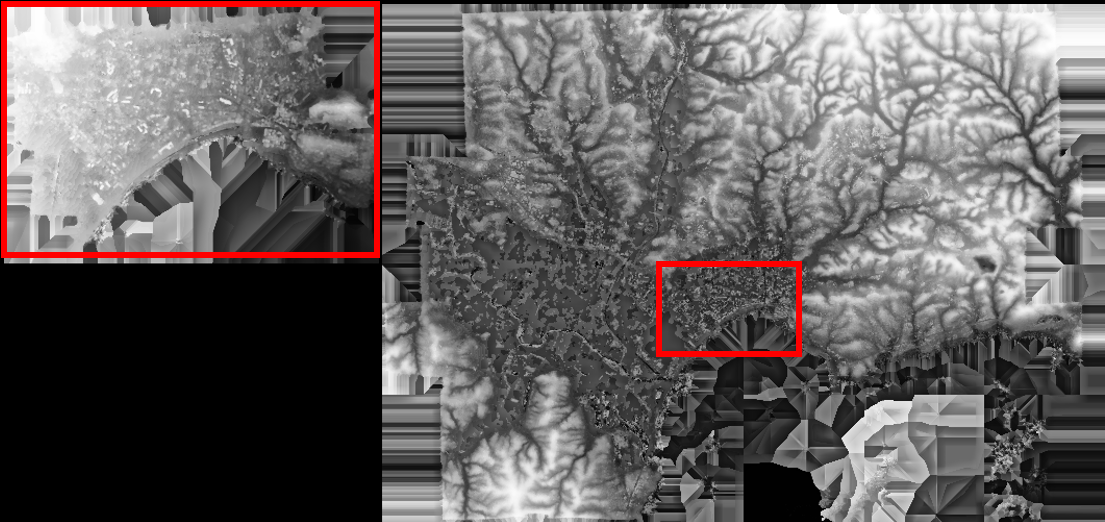
\includegraphics[width=7.8cm]{images/Chapitre3/MEC-Malt_Tapas_1970_MEC-Malt_2014.png}
			\end{minipage}%
		}
		\subfigure[Match number (DSM)]{
			\begin{minipage}[t]{0.35\linewidth}
				\centering
				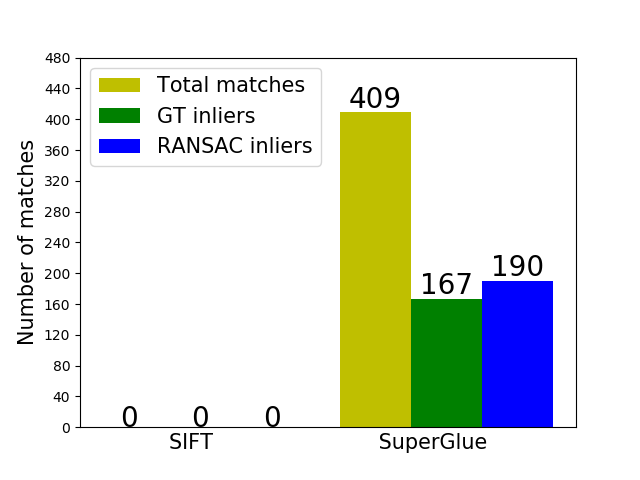
\includegraphics[width=4.8cm]{images/Chapitre3/PlotCurves_MEC-Malt_Tapas_1970_MEC-Malt_2014.png}
			\end{minipage}%
		}
		\subfigure[$SIFT_{DSM}$]{
			\begin{minipage}[t]{0.48\linewidth}
				\centering
				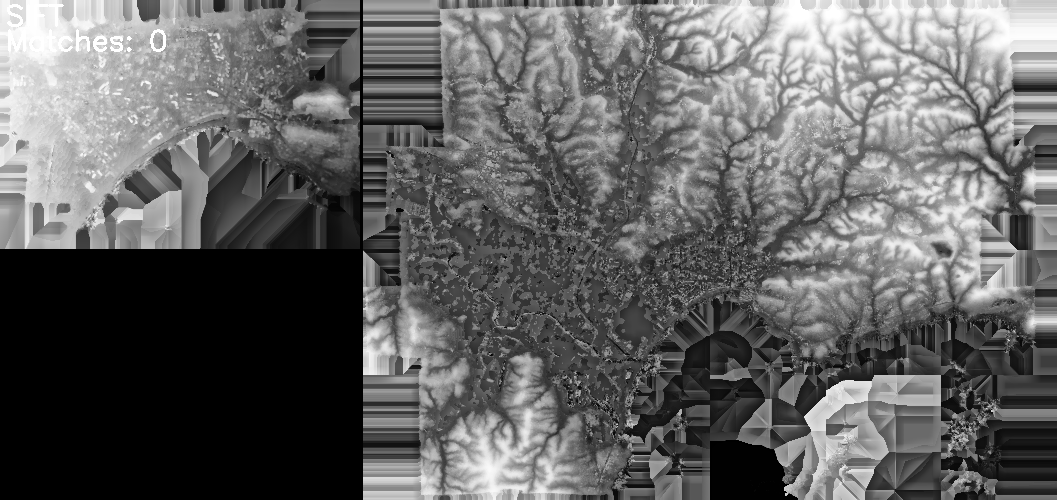
\includegraphics[width=6cm]{images/Chapitre3/Homol-SIFT-2DRANSAC_MEC-Malt_Tapas_1970_MEC-Malt_2014.png}
			\end{minipage}%
		}
		\subfigure[$SuperGlue_{DSM}$]{
			\begin{minipage}[t]{0.48\linewidth}
				\centering
				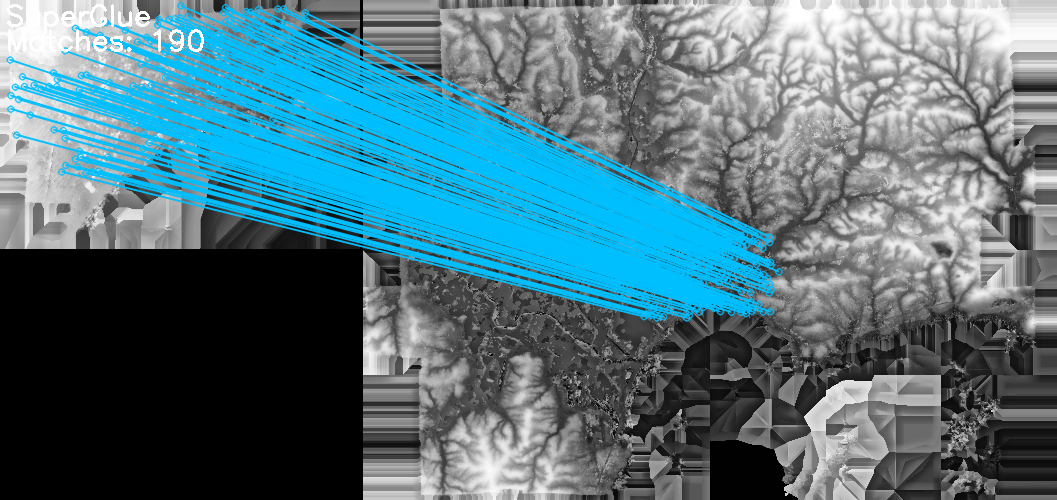
\includegraphics[width=6cm]{images/Chapitre3/Homol-SubPatch_R270-2DRANSAC_MEC-Malt_Tapas_1970_MEC-Malt_2014.png}
			\end{minipage}%
		}
		\caption{Result of matching DSMs of Fr{\'e}jus 1970 and 2014}
		\label{Match result}
	\end{center}
\end{figure*} 

\subsubsection{Ground check points}
We manually measured 3 GCPs as check points to evaluate the roughly co-registered orientations resulted by 6 methods:\\
\begin{enumerate}
	\item Match image pairs using SIFT;
	\item Match image pairs using SuperGlue;
	\item Match orthophotos using SIFT;
	\item Match orthophotos using SuperGlue;
	\item Match DSMs using SIFT;
	\item Match DSMs using SuperGlue;
\end{enumerate}

\begin{table}%[H]
	\footnotesize
	\centering
	\begin{tabular}{|l|c|c|c|c|c|c|}\hline
		&\multicolumn{6}{c|}{$|\mu|$ [m]}\\\hline
		&\multicolumn{2}{c|}{ImgPairs} &\multicolumn{2}{c|}{Orthophoto} &\multicolumn{2}{c|}{DSM}\\\hline
		& SIFT & SuperGlue & SIFT & SuperGlue & SIFT & SuperGlue \\\hline\hline
		$Frejus_{2014}^{1954}$ & 645.57 & 29.29 & / & 34.84 & / & \textbf{10.72}\\\hline
		$Frejus_{2014}^{1966}$ & 1346.35 & 18.15 & / & 11.98 & / & \textbf{10.43}\\\hline
		$Frejus_{2014}^{1970}$ & 2194.77 & 11.09 & / & 16.87 & / & \textbf{10.23}\\\hline\hline
		$Kobe_{1994}^{1991}$ & / & \textbf{0.761} & 0 & 1.2775 & 1.0465 & 1.5155\\\hline
\end{tabular}
	\caption{Accuracy of 6 sets of co-registered orientations resulting from 6 methods, evaluated on 3 check points uniformly distributed in the block. Absolute average value $|\mu|$ is displayed for each method.}
	\label{CheckptAcuracy}
\end{table}

\subsubsection{DoD}


\begin{figure*}[htbp]
	\begin{center}
		\subfigure[DoD$_{Frejus1954}^{ImgPairs}$]{
			\begin{minipage}[t]{0.31\linewidth}
				\centering
				%left, lower, right, up
				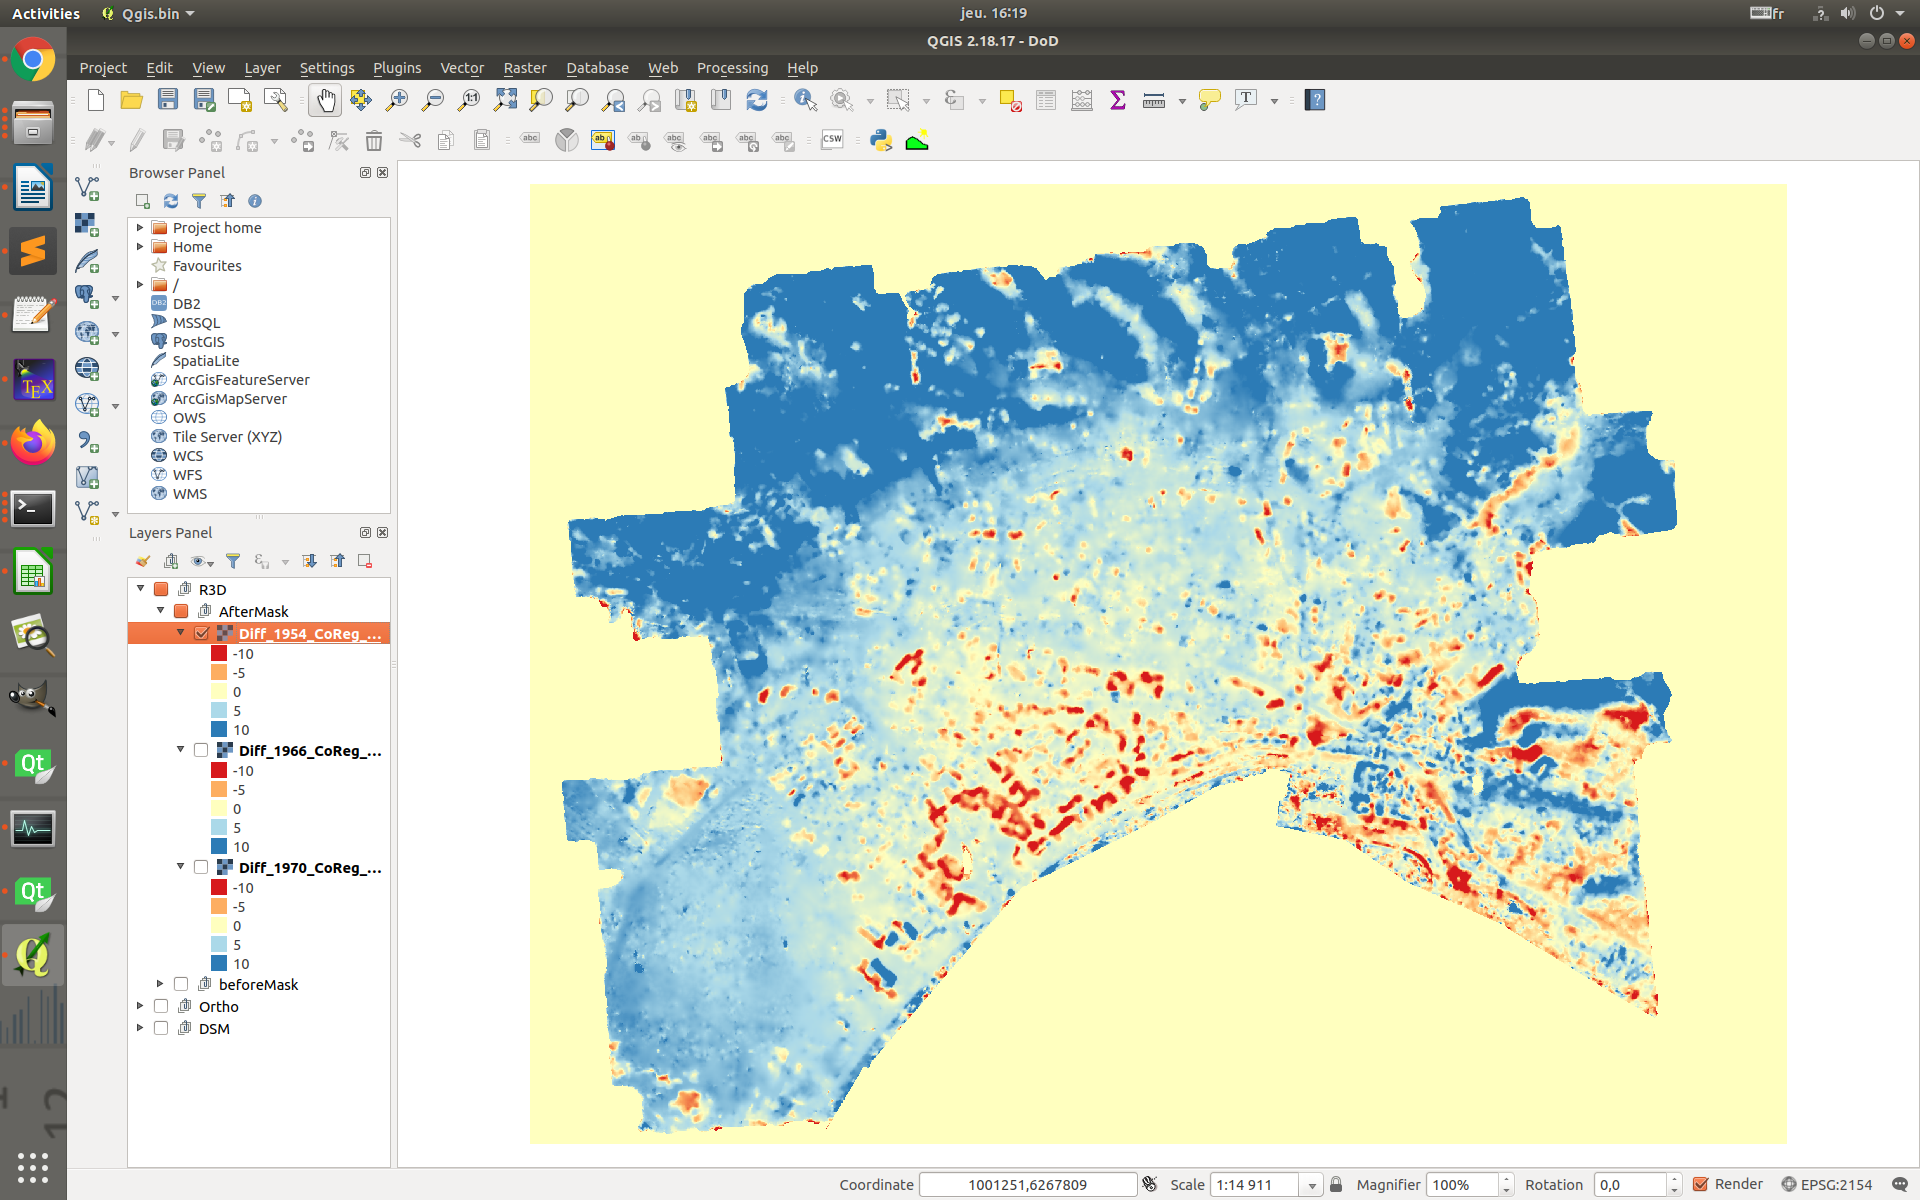
\includegraphics[width=4.2cm,trim=550 60 230 200,clip]{images/Chapitre3/DoD1954R3D.png}
			\end{minipage}%
		}
		\subfigure[DoD$_{Frejus1954}^{Orthophoto}$]{
			\begin{minipage}[t]{0.31\linewidth}
				\centering
				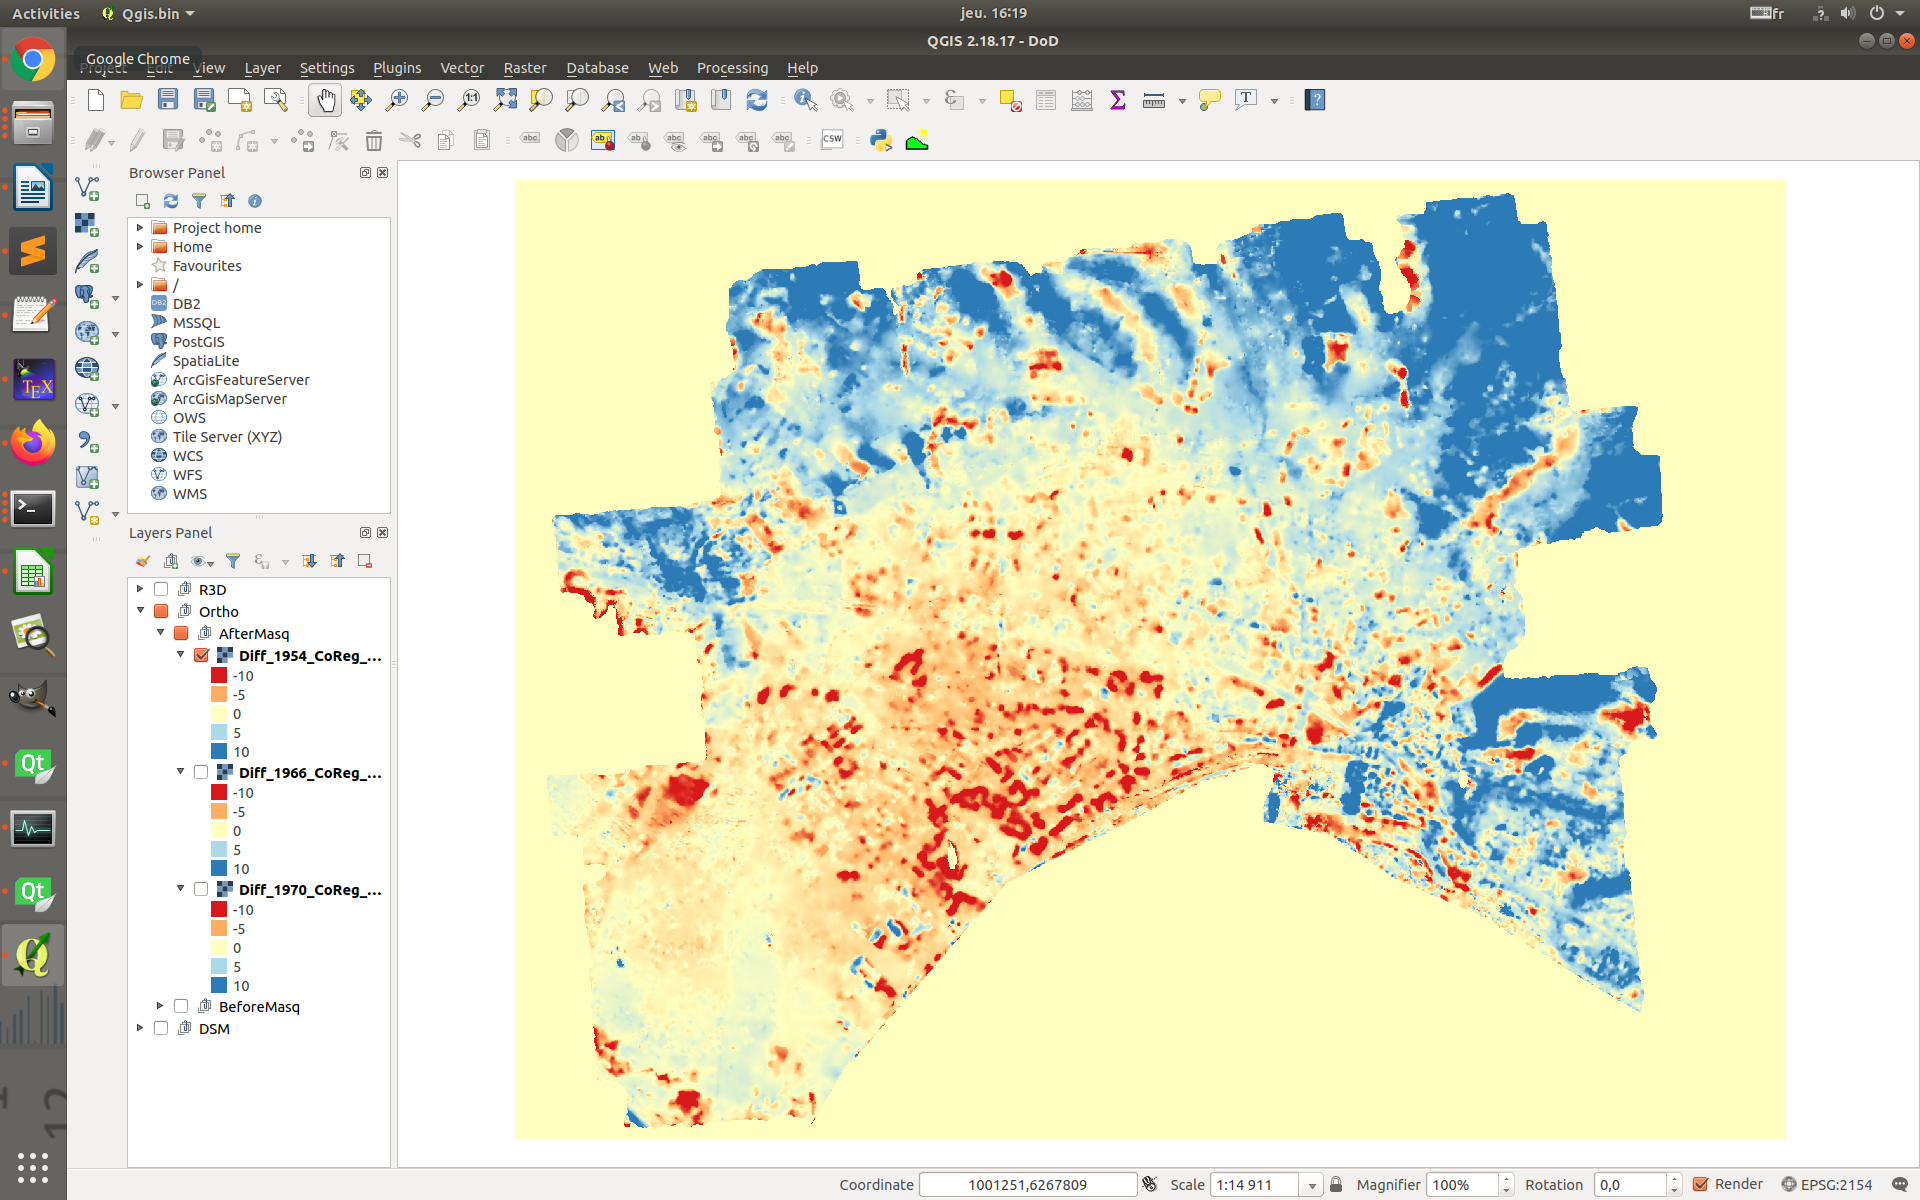
\includegraphics[width=4.2cm,trim=550 60 230 200,clip]{images/Chapitre3/DoD1954Ortho.png}
			\end{minipage}%
		}
		\subfigure[DoD$_{Frejus1954}^{DSM}$]{
			\begin{minipage}[t]{0.31\linewidth}
				\centering
				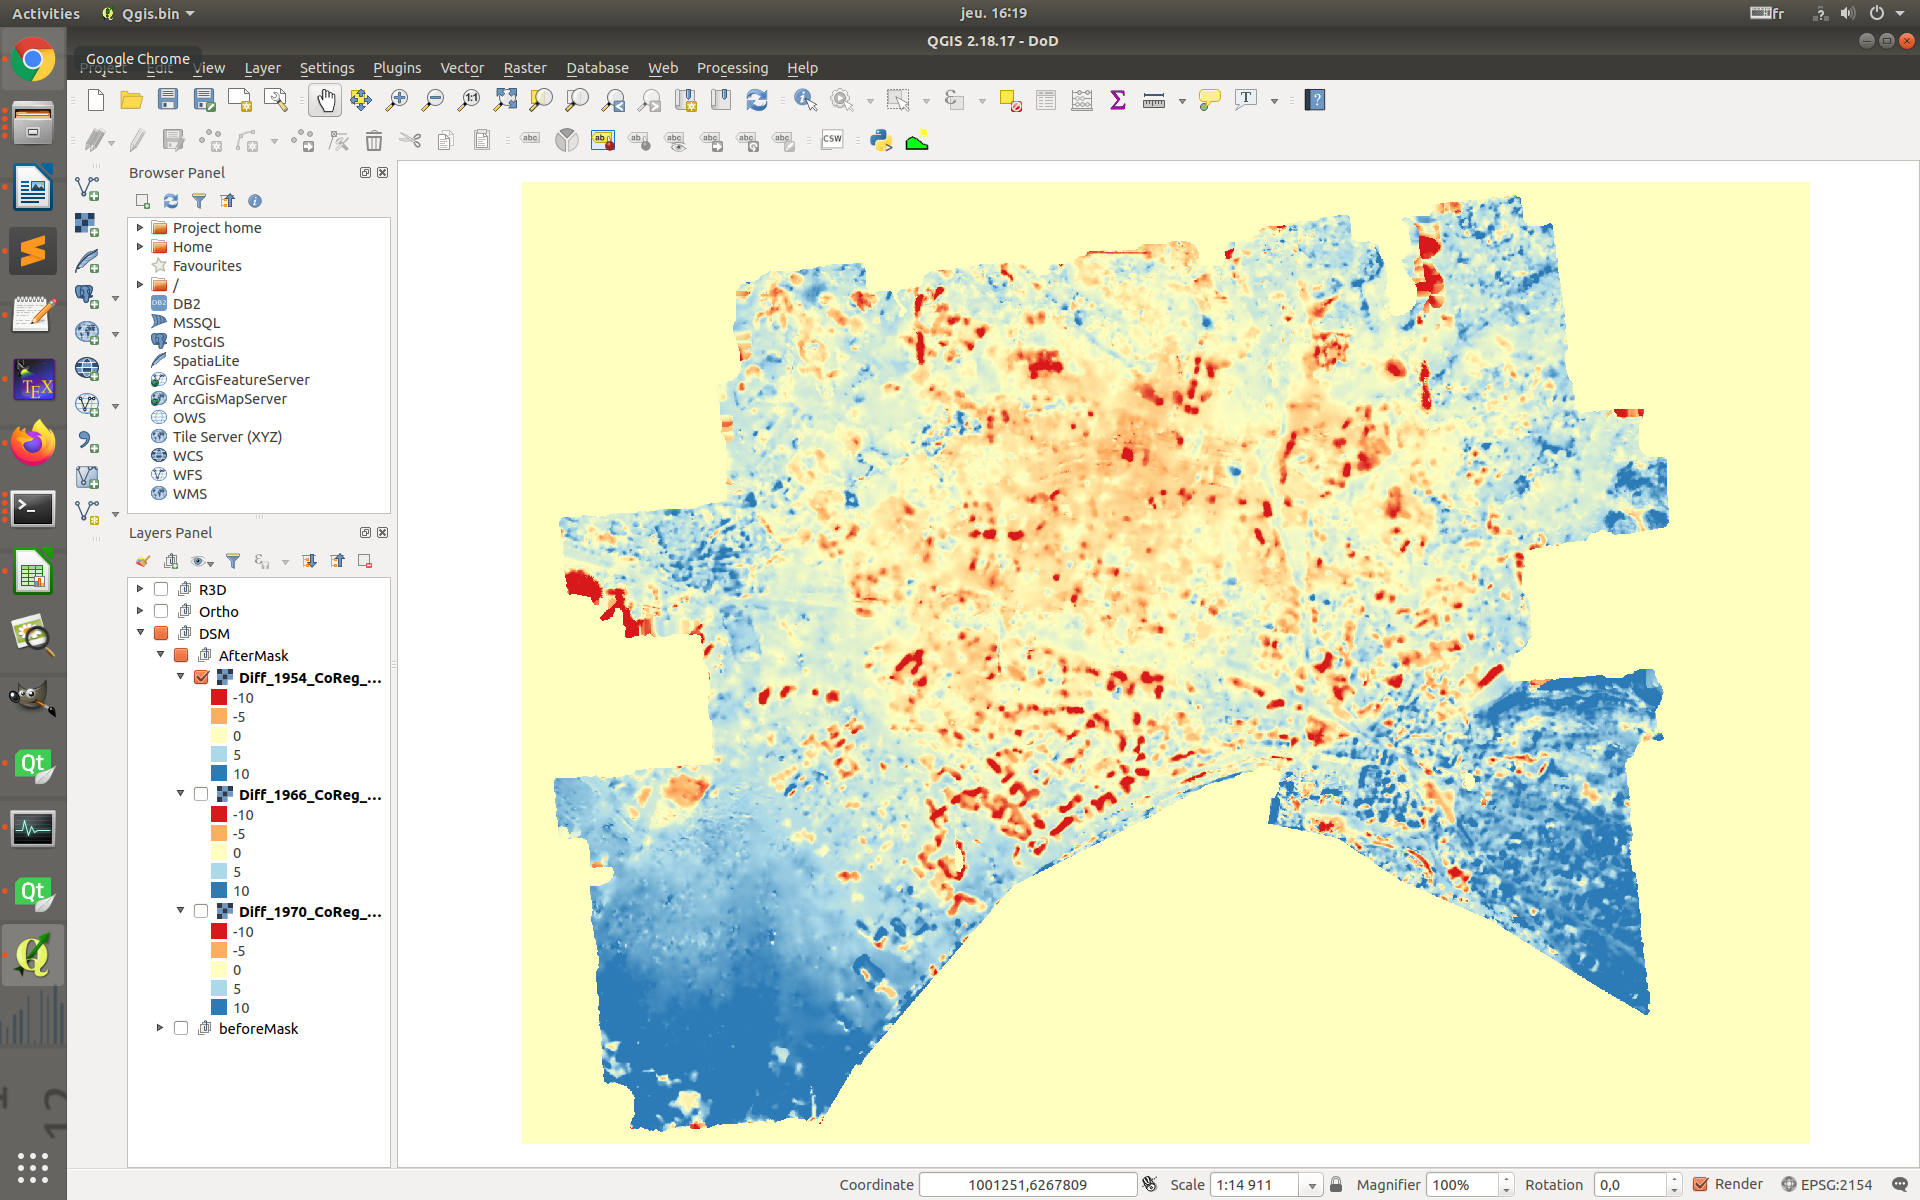
\includegraphics[width=4.2cm,trim=550 60 230 200,clip]{images/Chapitre3/DoD1954DSM.png}
			\end{minipage}%
		}
		
		\subfigure[DoD$_{Frejus1966}^{ImgPairs}$]{
			\begin{minipage}[t]{0.31\linewidth}
				\centering
				%left, lower, right, up
				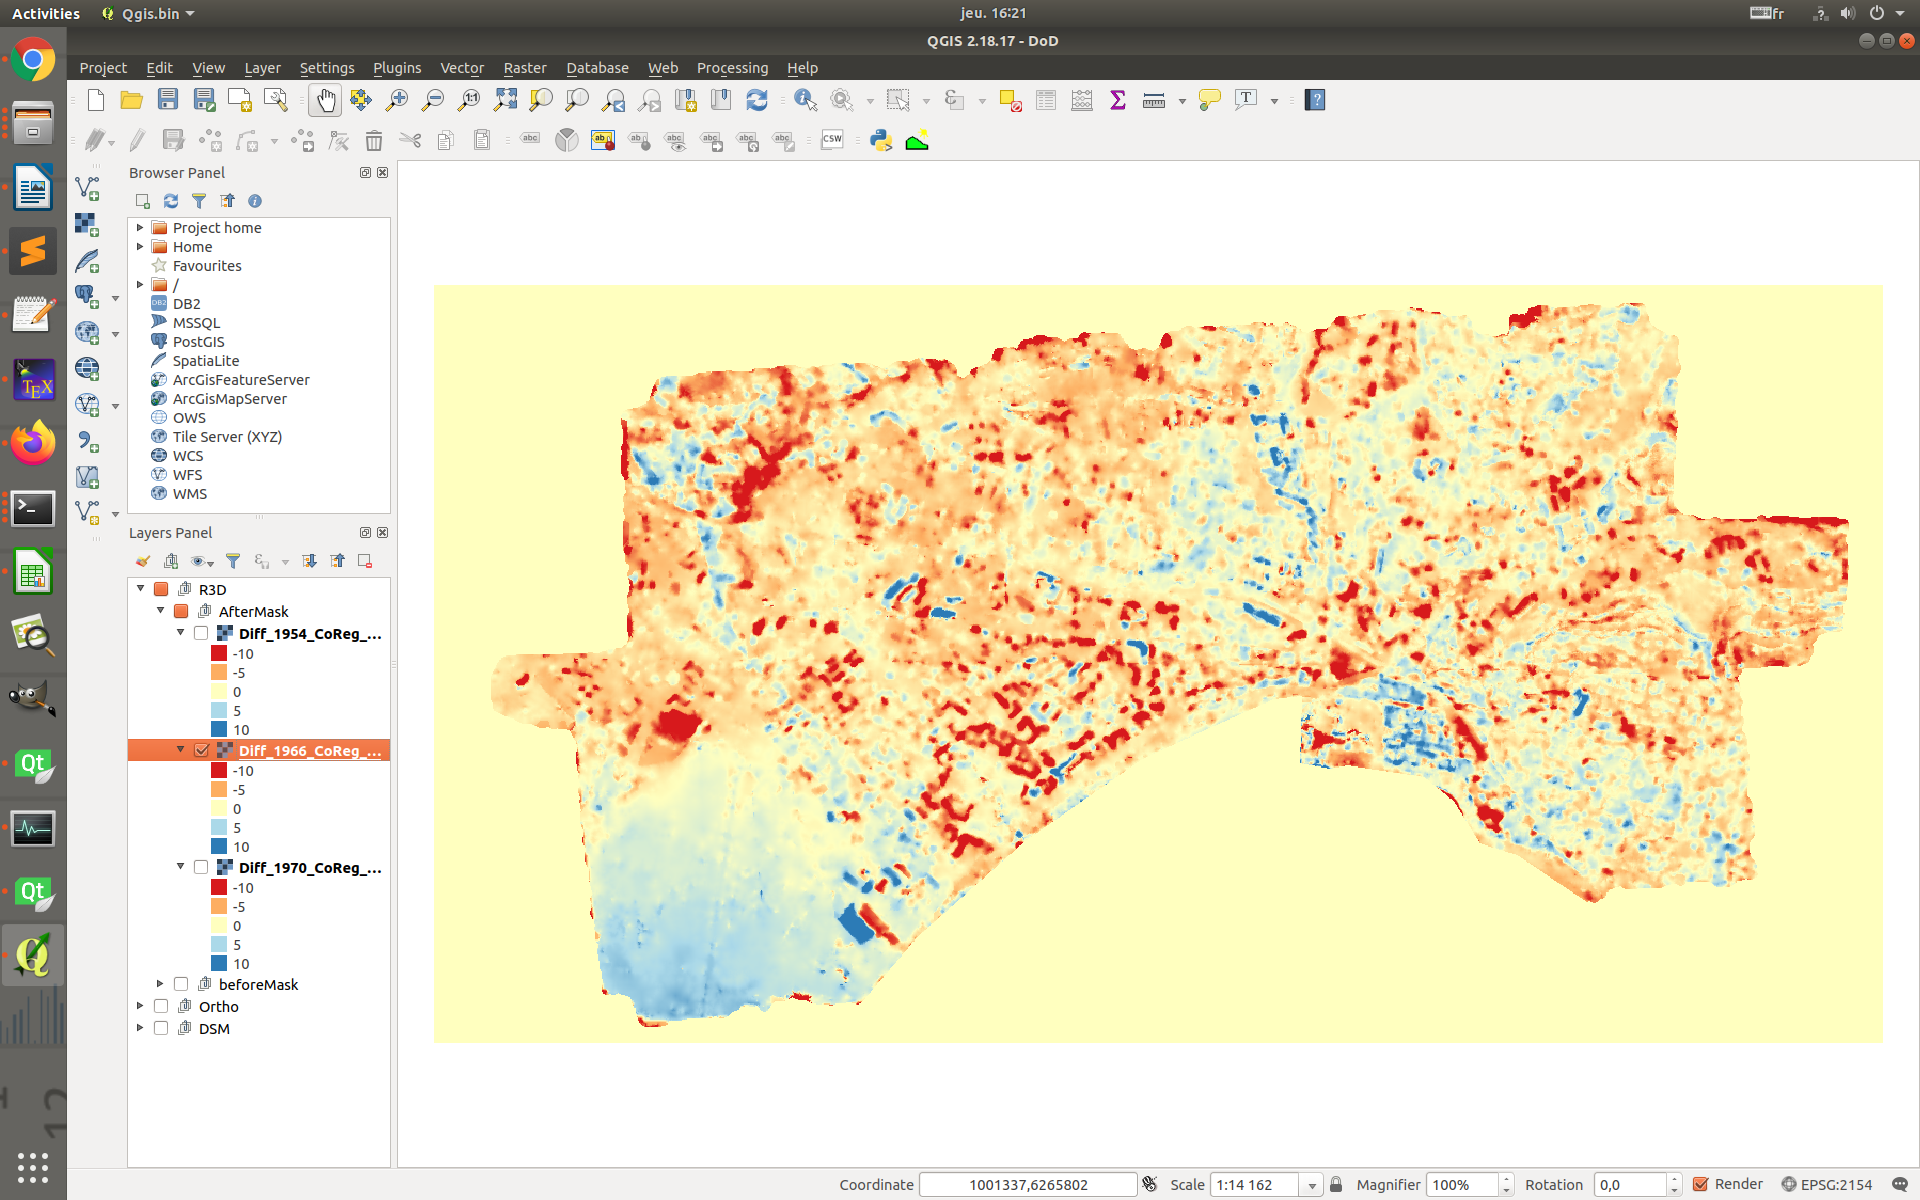
\includegraphics[width=4.2cm,trim=480 60 50 200,clip]{images/Chapitre3/DoD1966R3D.png}
			\end{minipage}%
		}
		\subfigure[DoD$_{Frejus1954}^{Orthophoto}$]{
			\begin{minipage}[t]{0.31\linewidth}
				\centering
				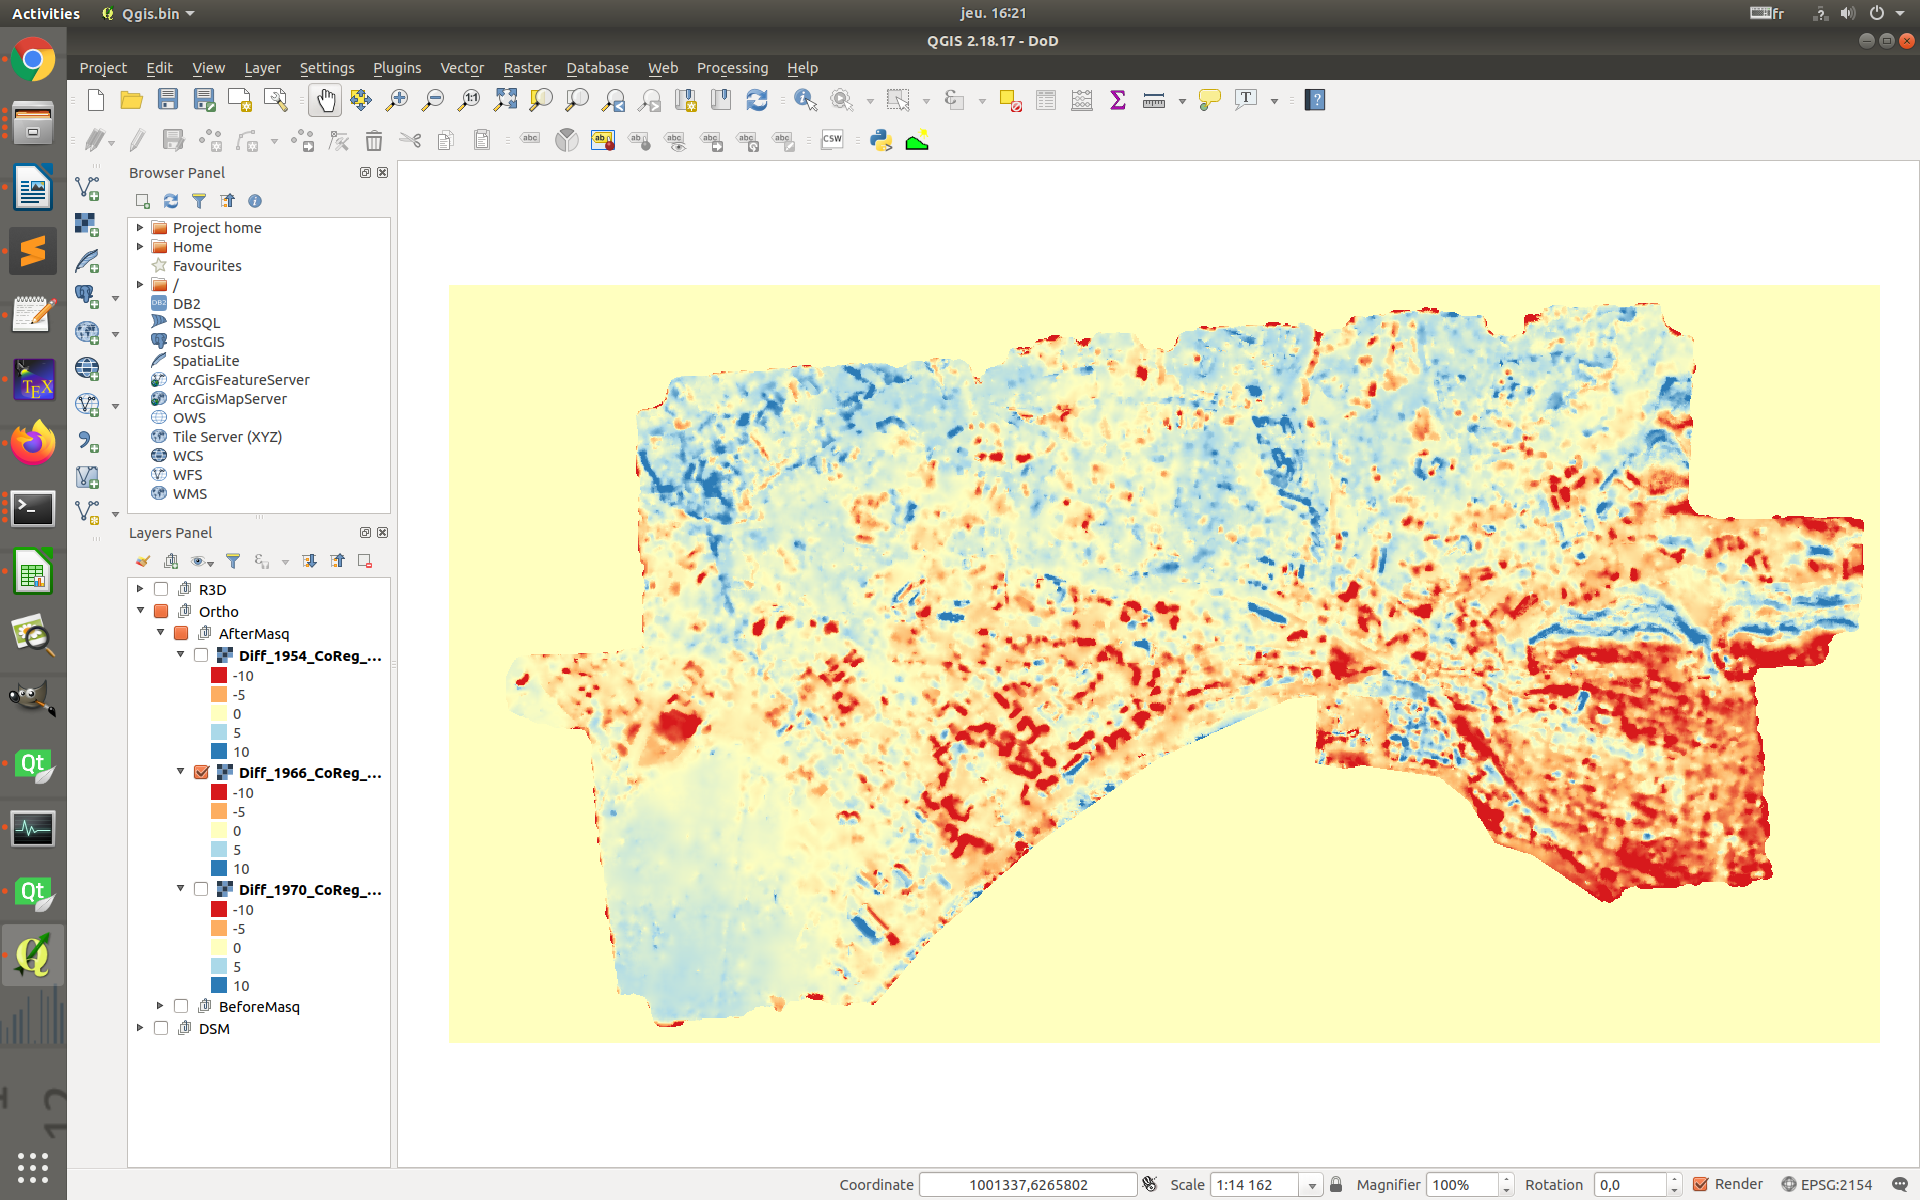
\includegraphics[width=4.2cm,trim=480 60 50 200,clip]{images/Chapitre3/DoD1966Ortho.png}
			\end{minipage}%
		}
		\subfigure[DoD$_{Frejus1966}^{DSM}$]{
			\begin{minipage}[t]{0.31\linewidth}
				\centering
				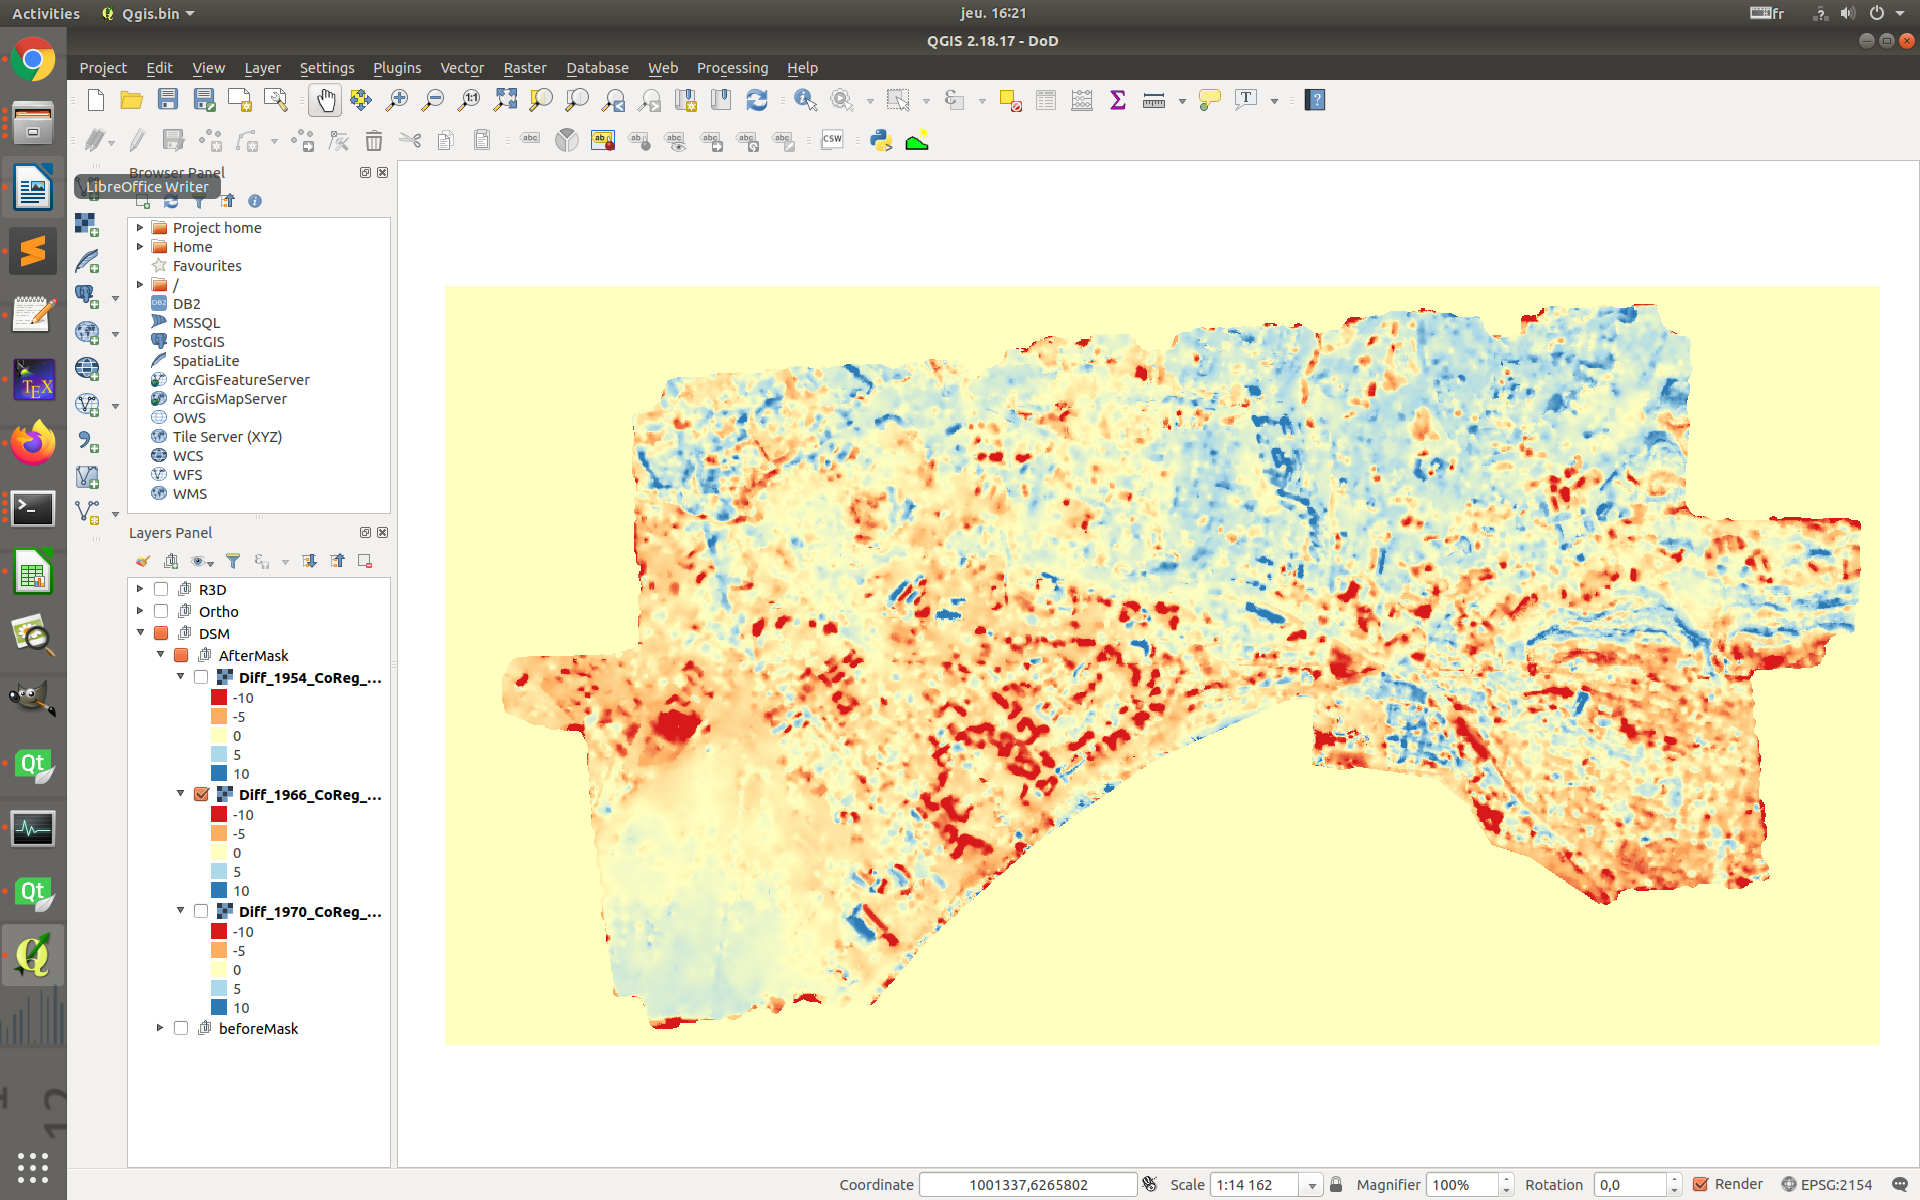
\includegraphics[width=4.2cm,trim=480 60 50 200,clip]{images/Chapitre3/DoD1966DSM.png}
			\end{minipage}%
		}
		
		\subfigure[DoD$_{Frejus1970}^{ImgPairs}$]{
			\begin{minipage}[t]{0.31\linewidth}
				\centering
				%left, lower, right, up
				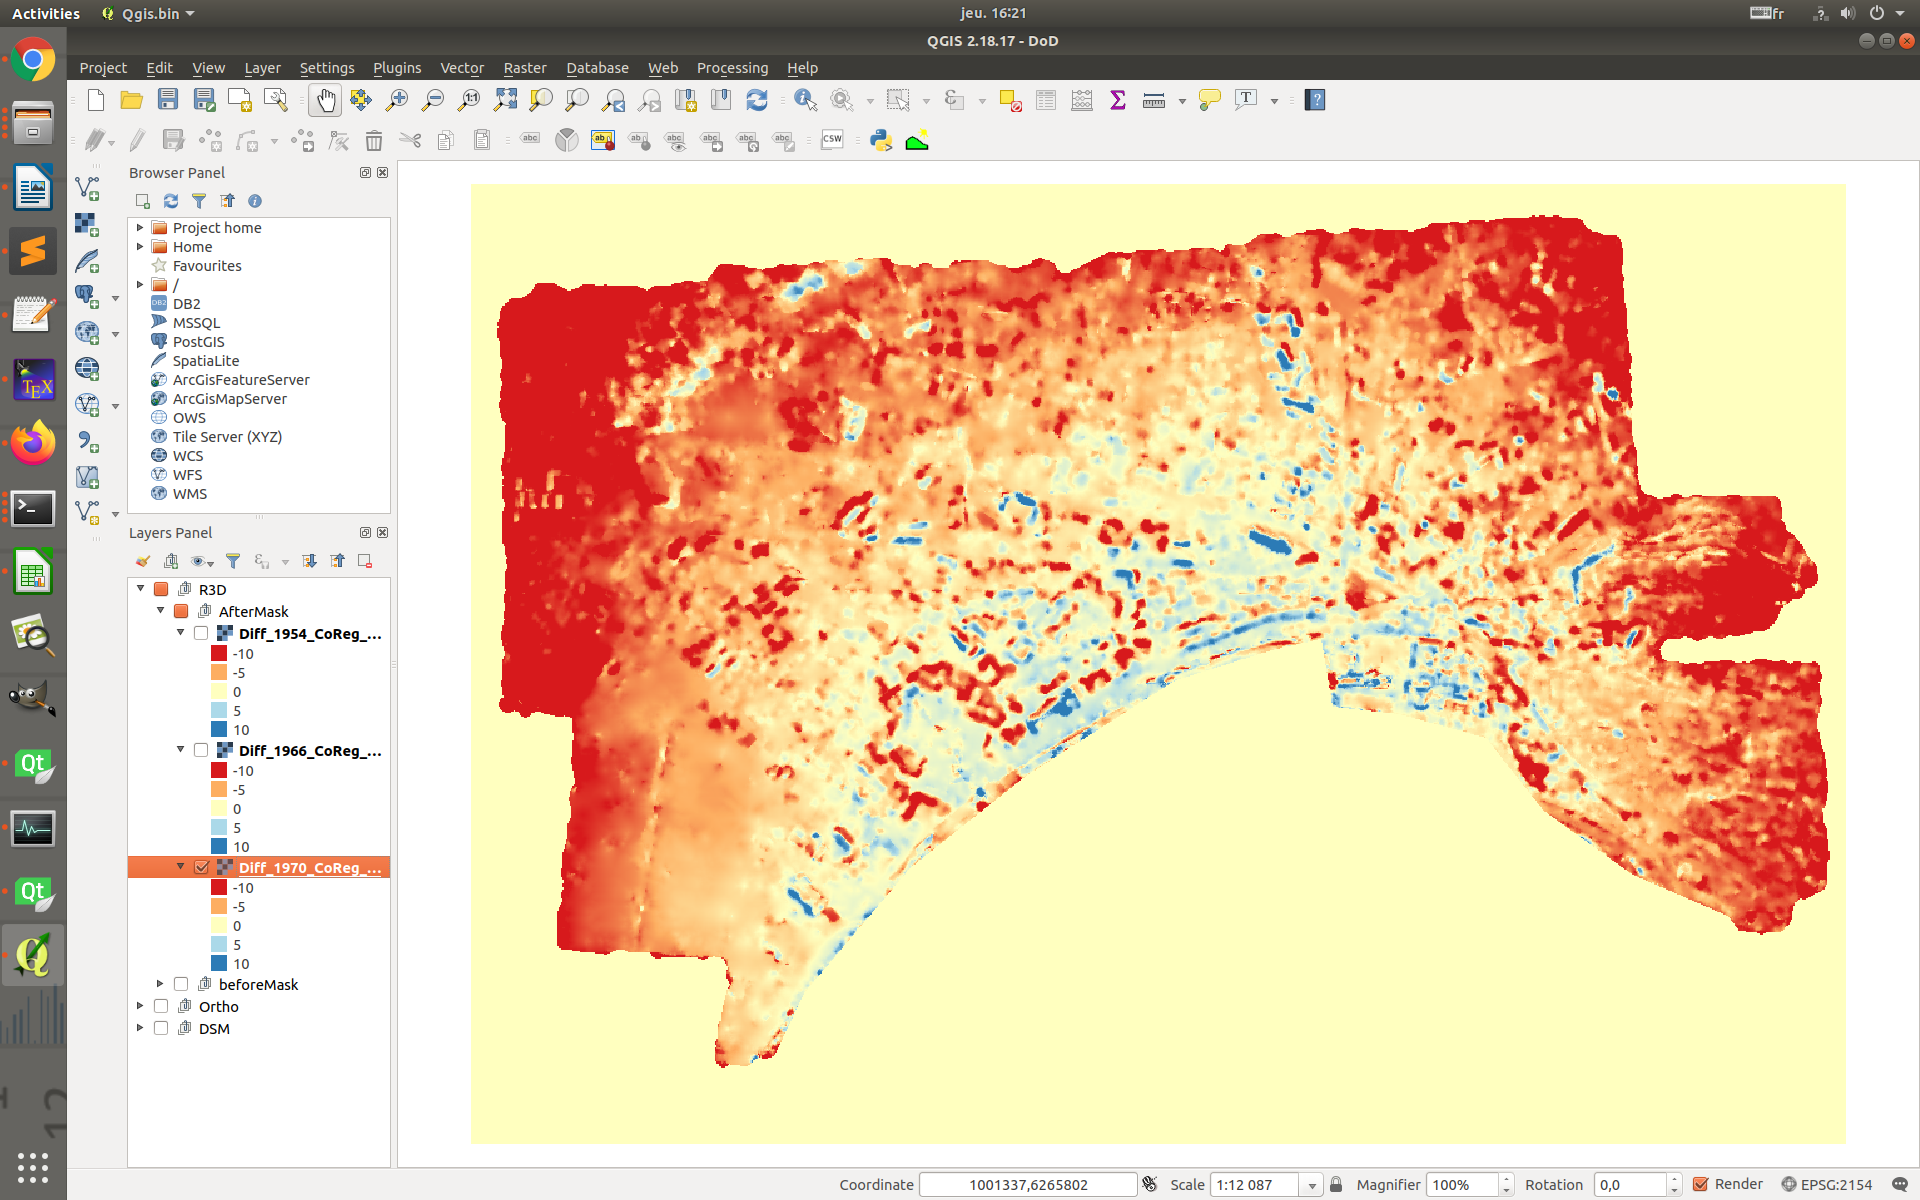
\includegraphics[width=4.2cm,trim=480 110 50 200,clip]{images/Chapitre3/DoD1970R3D.png}
			\end{minipage}%
		}
		\subfigure[DoD$_{Frejus1970}^{Orthophoto}$]{
			\begin{minipage}[t]{0.31\linewidth}
				\centering
				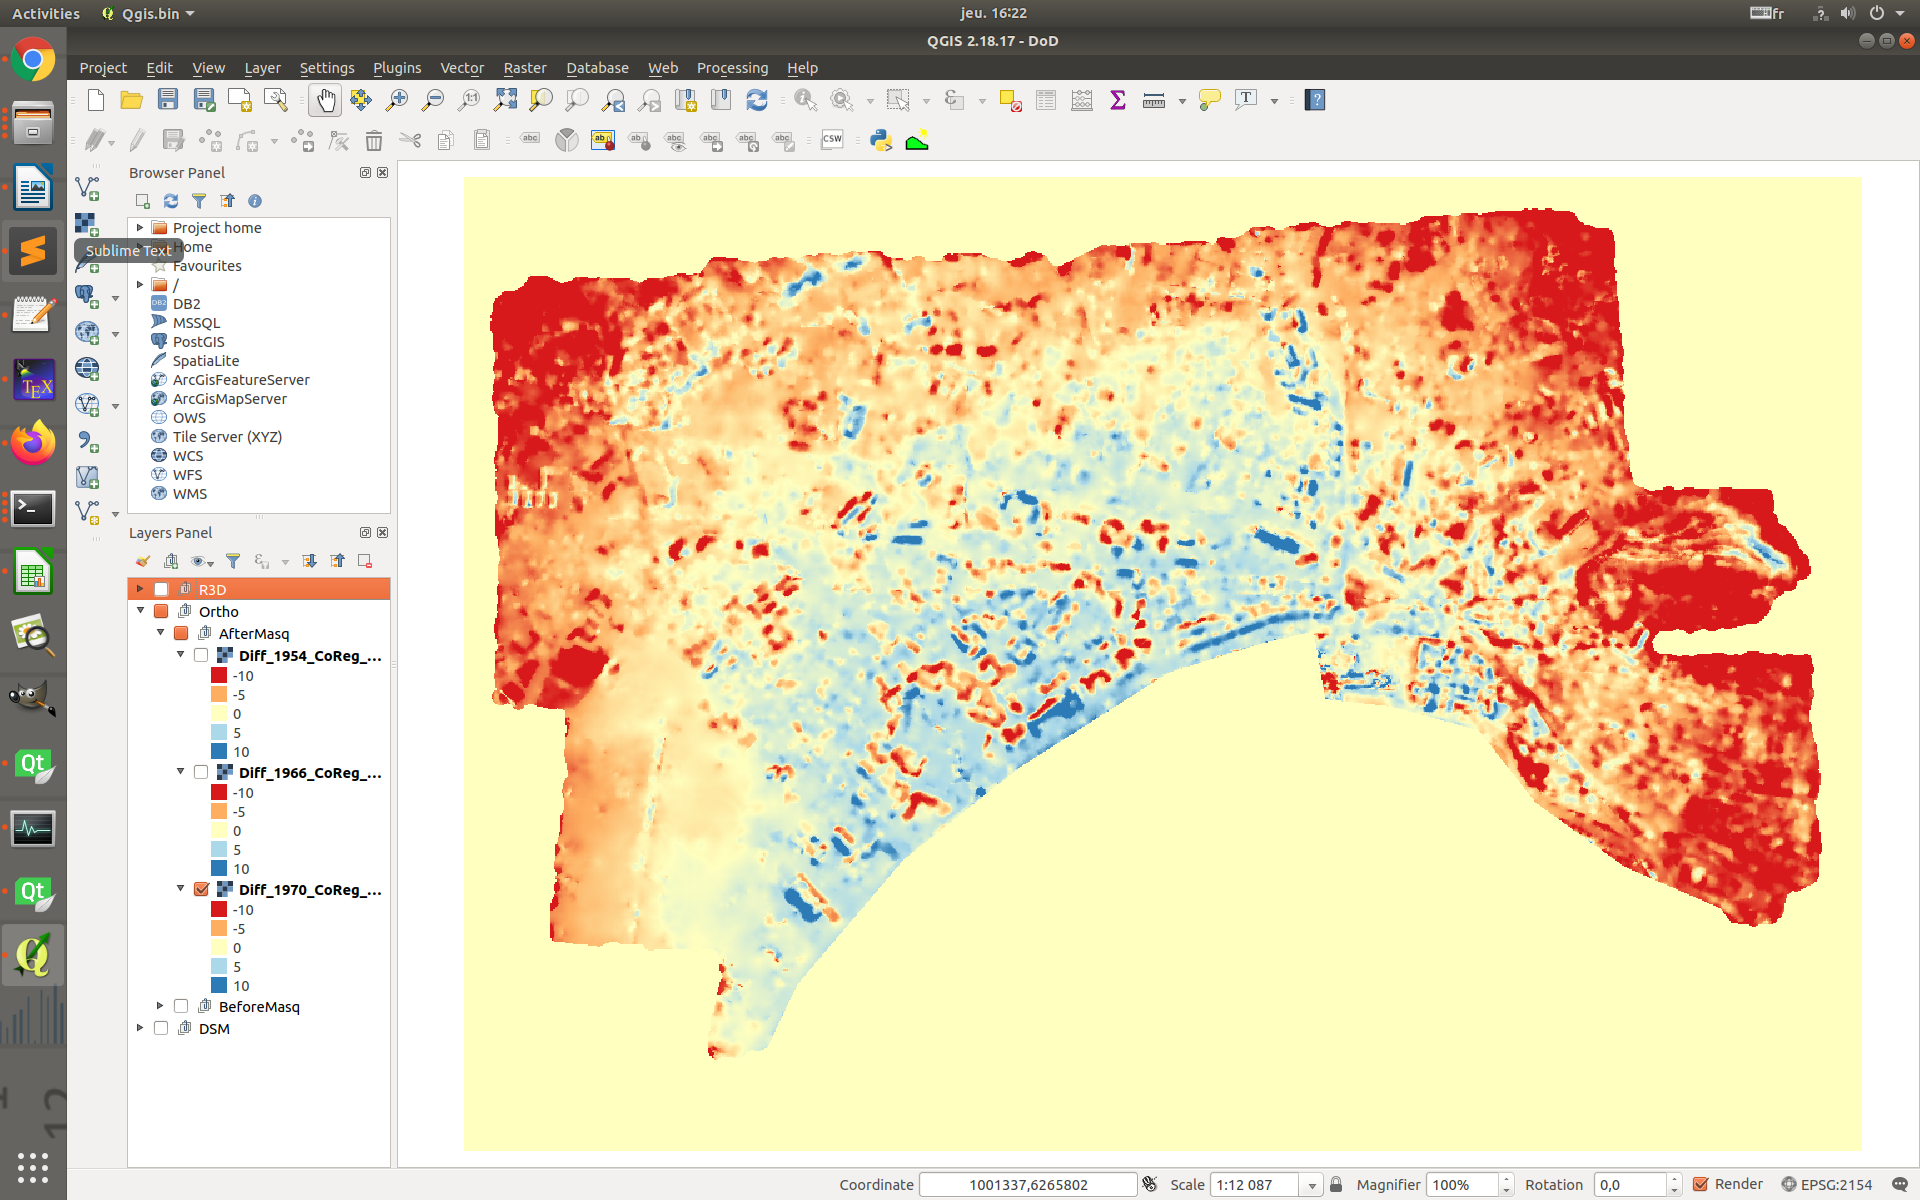
\includegraphics[width=4.2cm,trim=480 110 50 200,clip]{images/Chapitre3/DoD1970Ortho.png}
			\end{minipage}%
		}
		\subfigure[DoD$_{Frejus1970}^{DSM}$]{
			\begin{minipage}[t]{0.31\linewidth}
				\centering
				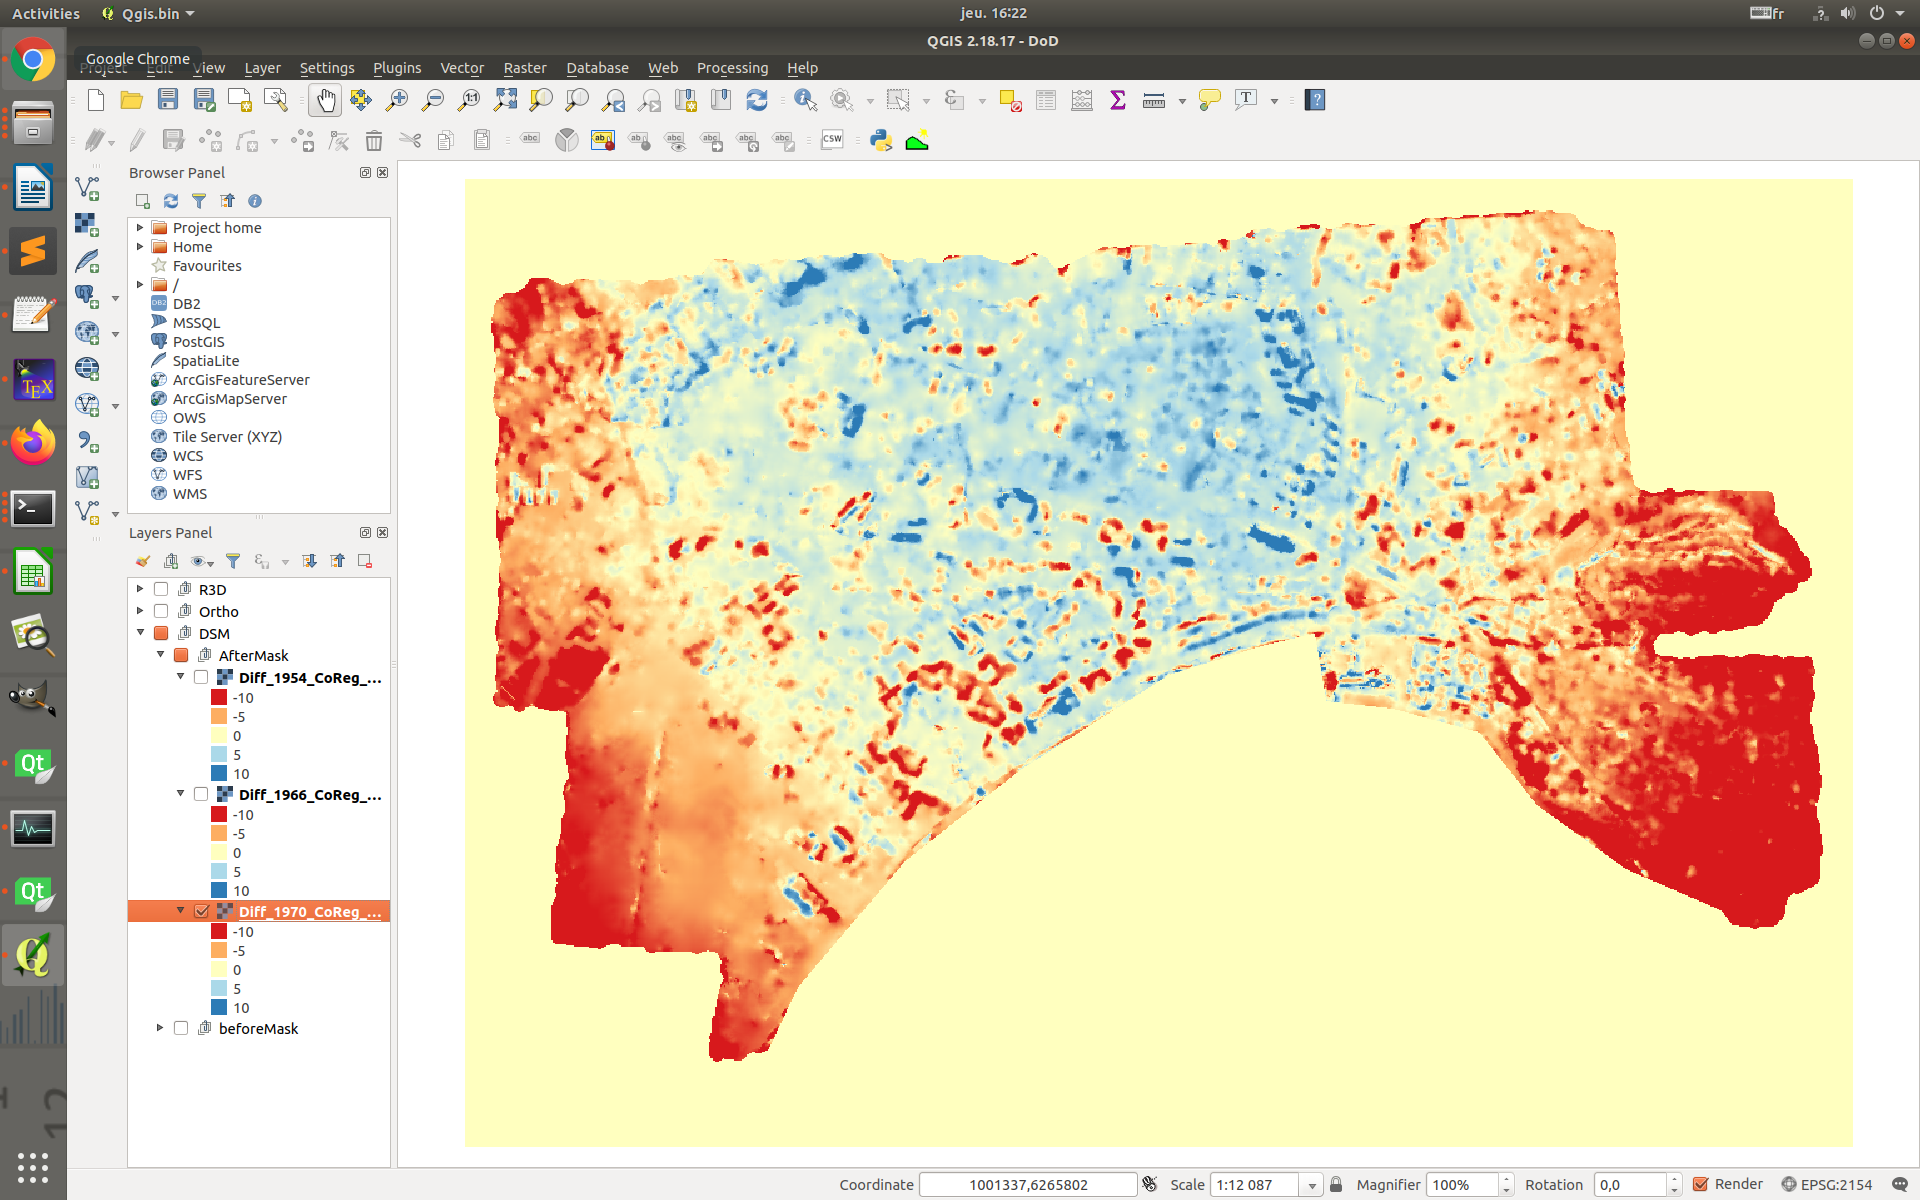
\includegraphics[width=4.2cm,trim=480 110 50 200,clip]{images/Chapitre3/DoD1970DSM.png}
			\end{minipage}%
		}
		
		\subfigure[DoD legend]{
			\begin{minipage}[t]{1\linewidth}
				\centering
				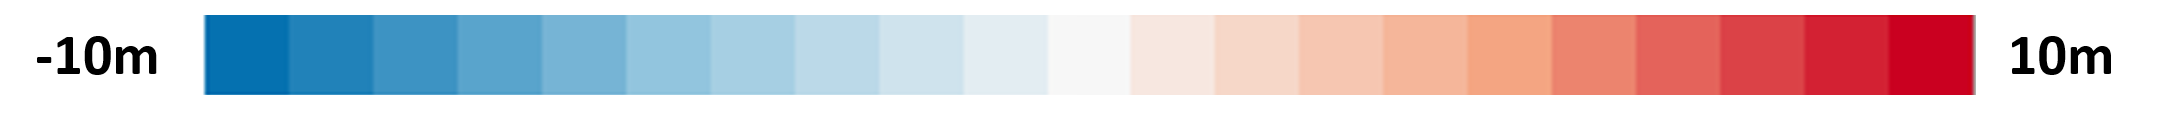
\includegraphics[width=11cm]{images/Chapitre3/LegendDoD.png}
			\end{minipage}%
		}
		\caption{DoDs of SuperGlue on dataset Fr{\'e}jus}
		\label{Frejus DoD of SuperGlue}
	\end{center}
\end{figure*} 

\begin{table}%[H]
	\footnotesize
	\centering
	\begin{tabular}{||l|c|c|c||}\hline
		&$\mu$ [m]&$\sigma$ [m]&$|\mu|$ [m]\\\hline\hline
		DoD$_{Frejus1954}^{ImgPairs}$ & 5.70 & 6.32 & 6.62\\
		DoD$_{Frejus1954}^{Orthophoto}$ & 2.19 & 6.46 & 4.55\\
		DoD$_{Frejus1954}^{DSM}$ & 2.07 & 4.87 & \textbf{3.83}\\\hline
		DoD$_{Frejus1966}^{ImgPairs}$ & -1.36 & 3.82 & 2.90\\
		DoD$_{Frejus1966}^{Orthophoto}$ & -0.37 & 4.22 & 3.01\\
		DoD$_{Frejus1966}^{DSM}$ & -0.46 & 3.77 & \textbf{2.68}\\\hline
		DoD$_{Frejus1970}^{ImgPairs}$ & -5.04 & 5.09 & 5.70\\
		DoD$_{Frejus1970}^{Orthophoto}$ & -2.63 & 5.18 & \textbf{4.39}\\
		DoD$_{Frejus1970}^{DSM}$ & -1.71 & 5.75 & 4.61\\\hline
	\end{tabular}
	\caption{Average value $\mu$, standard deviation $\sigma$, and absolute average value $|\mu|$ of all the DoDs in Figure~\ref{Frejus DoD of SuperGlue}.}
	\label{CheckptAcuracy}
\end{table}



%%%%%%%%%%%%%%%%%%%%%%%%%%%%%%%%%%%%%%

\begin{figure*}[htbp]
	\begin{center}
		\subfigure[Image pairs]{
			\begin{minipage}[t]{0.45\linewidth}
				\centering
				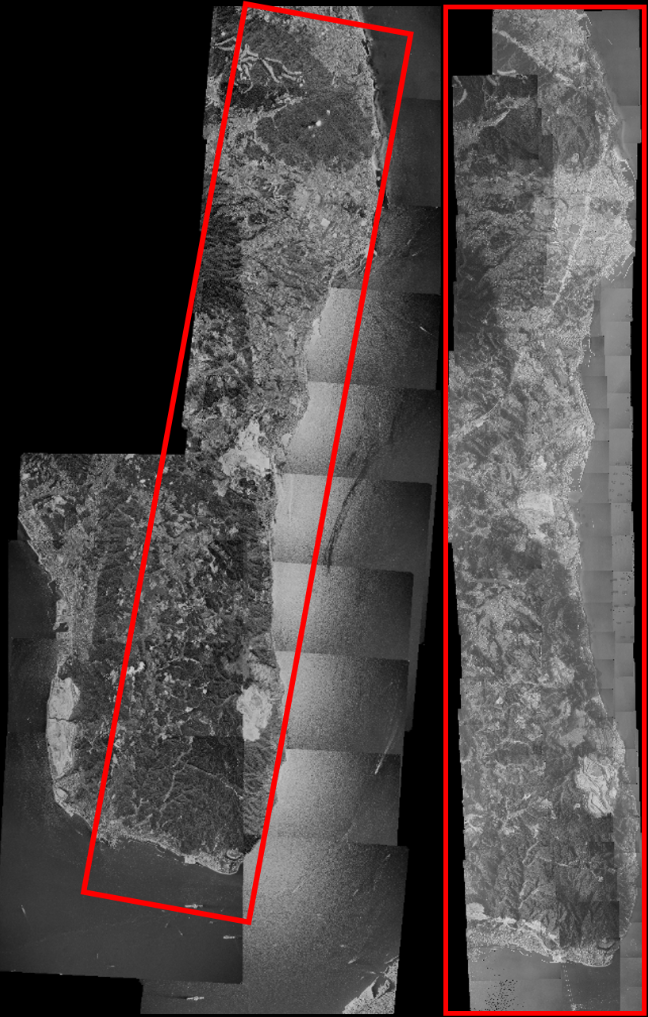
\includegraphics[width=5.5cm]{images/Chapitre3/Pseudo-Ortho-MEC-Malt_Tapas_1991_Ortho-MEC-Malt_Tapas_1994.png}
			\end{minipage}%
		}
		\subfigure[Match number (ImgPairs)]{
			\begin{minipage}[t]{0.35\linewidth}
				\centering
				\includegraphics[width=4.8cm]{images/Chapitre3/PlotCurves_Pseudo-Ortho-MEC-Malt_Tapas_1991_Ortho-MEC-Malt_Tapas_1994.png}
			\end{minipage}%
		}	
		\subfigure[$SIFT_{ImgPairs}$]{
			\begin{minipage}[t]{0.45\linewidth}
				\centering
				\includegraphics[width=5.5cm]{images/Chapitre3/Pseudo-Homol-SIFT2Step_1991-1994-Rough-2DRANSAC-GlobalR3D-PileImg_Ortho-MEC-Malt_Tapas_1991_Ortho-MEC-Malt_Tapas_1994.png}
			\end{minipage}%
		}
		\subfigure[$SuperGlue_{ImgPairs}$]{
			\begin{minipage}[t]{0.45\linewidth}
				\centering
				\includegraphics[width=5.5cm]{images/Chapitre3/Pseudo-Homol-SuperGlue_1991-1994-GlobalR3D-PileImg_Ortho-MEC-Malt_Tapas_1991_Ortho-MEC-Malt_Tapas_1994.png}
			\end{minipage}%
		}
		\caption{Result of matching image pairs of Kobe 1991 and 1995}
		\label{Match result}
	\end{center}
\end{figure*} 

\begin{figure*}[htbp]
	\begin{center}
		\subfigure[Orthophotos]{
			\begin{minipage}[t]{0.45\linewidth}
				\centering
				\includegraphics[width=5.5cm]{images/Chapitre3/Ortho-MEC-Malt_Tapas_1991_Ortho-MEC-Malt_Tapas_1994.png}
			\end{minipage}%
		}
		\subfigure[Match number (ortho)]{
			\begin{minipage}[t]{0.35\linewidth}
				\centering
				\includegraphics[width=4.8cm]{images/Chapitre3/PlotCurves_Ortho-MEC-Malt_Tapas_1991_Ortho-MEC-Malt_Tapas_1994.png}
			\end{minipage}%
		}	
		\subfigure[$SIFT_{ortho}$]{
			\begin{minipage}[t]{0.45\linewidth}
				\centering
				\includegraphics[width=5.5cm]{images/Chapitre3/Homol-SIFT-2DRANSAC_Ortho-MEC-Malt_Tapas_1991_Ortho-MEC-Malt_Tapas_1994.png}
			\end{minipage}%
		}
		\subfigure[$SuperGlue_{ortho}$]{
			\begin{minipage}[t]{0.45\linewidth}
				\centering
				\includegraphics[width=5.5cm]{images/Chapitre3/Homol-SubPatch-2DRANSAC_Ortho-MEC-Malt_Tapas_1991_Ortho-MEC-Malt_Tapas_1994.png}
			\end{minipage}%
		}
		\caption{Result of matching orthophotos of Kobe 1991 and 1995}
		\label{Match result}
	\end{center}
\end{figure*} 

\begin{figure*}[htbp]
	\begin{center}
		\subfigure[DSMs]{
			\begin{minipage}[t]{0.45\linewidth}
				\centering
				\includegraphics[width=5.5cm]{images/Chapitre3/MEC-Malt_Tapas_1991_MEC-Malt_Tapas_1994.png}
			\end{minipage}%
		}
		\subfigure[Match number (DSM)]{
			\begin{minipage}[t]{0.35\linewidth}
				\centering
				\includegraphics[width=4.8cm]{images/Chapitre3/PlotCurves_MEC-Malt_Tapas_1991_MEC-Malt_Tapas_1994.png}
			\end{minipage}%
		}
		\subfigure[$SIFT_{DSM}$]{
			\begin{minipage}[t]{0.45\linewidth}
				\centering
				\includegraphics[width=5.5cm]{images/Chapitre3/Homol-SIFT-2DRANSAC_MEC-Malt_Tapas_1991_MEC-Malt_Tapas_1994.png}
			\end{minipage}%
		}
		\subfigure[$SuperGlue_{DSM}$]{
			\begin{minipage}[t]{0.45\linewidth}
				\centering
				\includegraphics[width=5.5cm]{images/Chapitre3/Homol-SubPatch-2DRANSAC_MEC-Malt_Tapas_1991_MEC-Malt_Tapas_1994.png}
			\end{minipage}%
		}
		\caption{Result of matching DSMs of Kobe 1991 and 1995}
		\label{Match result}
	\end{center}
\end{figure*} 


\section{Conclusion}

\section{Discussion}
